\documentclass{mcmthesis}
\bibliographystyle{plain}
\mcmsetup{CTeX = false,   % 使用 CTeX 套装时,设置为 true
        tcn = H155, problem = E,
        sheet = true, titleinsheet = true, keywordsinsheet = true,
        titlepage = false, abstract = true}
\usepackage{palatino}
\usepackage{lipsum}
\usepackage[UTF8, nocap]{ctex}
\usepackage{array}
\usepackage{float}
\usepackage{booktabs}
\usepackage{multirow}
\usepackage{subfigure}
\usepackage{longtable}

%\usepackage{ctex}
%\usepackage{CJK}
\title{Stable State Needed: a Glimpse of Climate Change Potency in Regional Fragility}
\author{}
\date{\today}

\begin{document}

	\begin{abstract}
		
		With the advancement of technology, the world has become less war and violence, and climate change is one of the most pervasive global threats to peace and security in the 21st century. In order to sovle these problem, we first propose an evaluation model to measure the fragility of worldwide countries. Then we apply Yemen and Gabon to show their instability. Last but not least, we take human interventions into consideration and modify our model to different regional scale.
		
		Firstly, 55 primary indicators are taken into consideration under the guide of four principles which is Society, Economics, Politics and Climate. And \textbf{Principal Component Analysis (PCA)} and \textbf{Entropy Weight Method(EWM)} are used to reduce indicator numbers and weight these indicators.
		
		Secondly, \textbf{Multiplier Model is proposed to anaylsis the indirect impact of climate change on fragility through interacting with indicators.} Then we determined the direct impact of climate: Disaster, Arable land, Forest and indirect impact: precipitation, cereal production and extreme temperatures.
		
		And we use \textbf{CFSFDP which is a clustering algorithm considering density peak to identify the tipping point.} The conclusion is that a country will reaches the tipping point when fragility index increase to 89.5, and it will probably fall into fragile state.
		
		Next, \textbf{we select Yemen and Gabon as research objects and analysis their fragility situation and reveal the impact of climate change both directly and indirectly.} As for Yemen, a fragile country, the fragility decrease from 96.3 to 80.18 without climate change. And for Gabon, a vulnerable country, Forest is the main risk to push it to fragile state. \textbf{An optimaization model is developed to minimize the total cost to prevent fragility}, and the results is that 22.3\% of its GDP which is about 3 billion dollars is needed for Gabon.
		
		At least, \textbf{our model is modified to fit the different regional scale.} For smaller and larger states, the factors, data and weights have reconsidered in order to make the model more comprehensive.
		
		
		
		\begin{keywords}
			Climate change; Fragility, EWM, Clustering, Optimization 
		\end{keywords}
	\end{abstract}

	\maketitle
	\setcounter{tocdepth}{2}
	\tableofcontents
	
	
	\section{Introduction}
	
		\subsection{Background}
		
			With the advancement of technology, the world has become less war and violence, But conflicts around the world have remained high for centuries. Climate change is one of the most pervasive global threats to peace and security in the 21st century. At the same time, there has been increasing acknowledgement within the academic literature and among the policy community of the relationship between climate change and security. The Intergovernmental Panel on Climate Change (IPCC) highlighted its latest report that human security will be progressively threatened as the climate changes.
	
		\subsection{Problem Restatement and Analysis}
			
			Since climate change is essential to state fragility, it is significant to propose an efficient model to give plans to detect and further predict the climate change poses in this problem. Therefore, index system is needed to evaluate the fragility of a region firstly. Two specific countries are selected to assess their fragility and effect of climate change through the index system. Then we have to propose feasible plans to help the fragile state get rid of the unfortunate situation and help countries that are vulnerable to maintain the status and further stabilise it. Moreover, the cost of human intervention should be considered in this problem. Eventually, We need to make sure the model works well in different regional scale sizes.
			
			This article is about a regional stability issue of in the worldwide, especially the impact of the climate change. We aim to design a measuring system to detect and predict how climate is and will change the regional fragility based on large quantities of data.Through the above analysis, the flow chart of this paper is shown in Figure \ref{fig:flowchart} as follows.
			
			\begin{figure}[h]
				\small
				\centering
				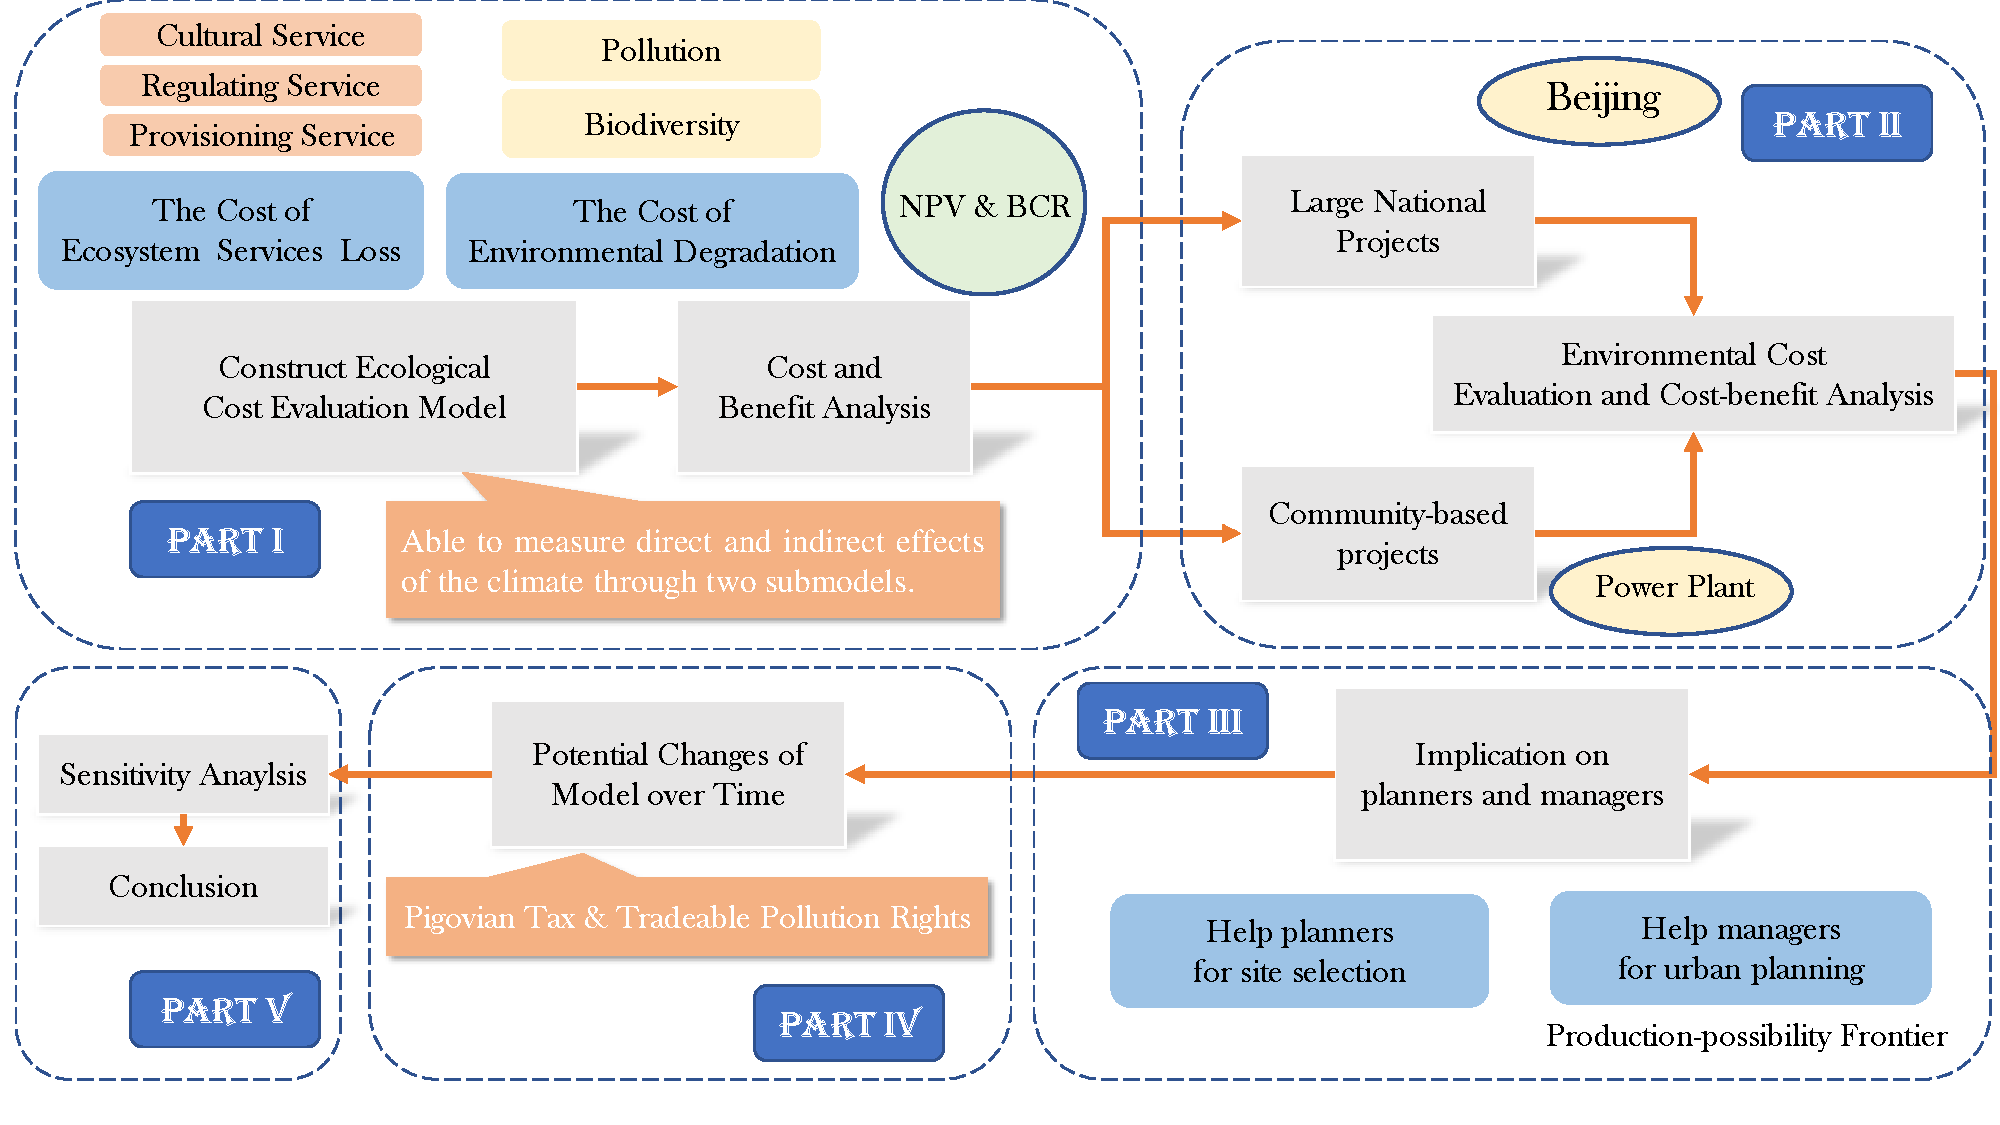
\includegraphics[width=14cm]{flowchart.pdf}
				\caption{The flow chart in this paper}
				\label{fig:flowchart}
			\end{figure}

		
		\subsection{Main Assumptions}
		
			\begin{itemize}
				\item We only consider the short-term effects of climate change. The long-term impact of climate change on a country's vulnerability is a very complex causal chain that is difficult to detect in a systematic, quantitative manner.
				
				\item There is no interaction between climate impact factors.
				
				\item Climate change can directly affect a country's fragility, and it can also implicit affect it by affecting other indicators. This effect can coexist.
			\end{itemize}

	
	\section{Preliminaries}
		\subsection{Terms and Mathematical Notations}
		
		In order to be clear and consistent through the paper, we now settle down some terms	and mathematical notations:
		
		\begin{table}[h]
			\caption{Symbol Table}
			\centering
			\renewcommand\arraystretch{1.32}
			\begin{tabular}{c l}
				\hline
				Symbol & Definition\\
				\noalign{\global\arrayrulewidth1pt}\hline\noalign{\global\arrayrulewidth0.9pt}
				AL & Arable land(synthetic action of precipitation and temperature) \\
				FA &	Forest area( the size of forest cover) \\
				DI &	the number of  disasters that have happened in current ten years \\
				GTI &	the degree of government transparency\\
				PLC &	the degree of political competition\\
				GDP &	GDP( the sum of the total value of the final products)\\
				GNI &	GNI per capita, PPP\\
				IH &	 the rate of intentional homicides happened per 100,000 people \\
				DCBN &	Cause of death, by non-communicable diseases\\ 
				MYOS &	Mean-years-of-schooling( the average annual enrolment rate )\\
				\hline
				
			\end{tabular}
		\end{table}
	
		\subsection{Data Pre-processing}
		
			\subsubsection{Data Collection}
				Collecting sufficient data is the basis of developing a complete index system. We searched the database and found 88 indicators of about three hundreds countries firstly. Most of the data come from the World Bank
				\footnote{https://data.worldbank.org/indicator
				}
				, and some data comes from NASA 
				\footnote{https://climate.nasa.gov/vital-signs/sea-level/}
				and OWID(Our World In Data)
				\footnote{https://ourworldindata.org/charts}
				, which is an publication that presents empirical data developed at the University of Oxford.
				
			\subsubsection{Data Filling}
				
				It is crucial that all data presented are authentic and easily verifiable. No model can provide stable assessments if based on unreliable or untruthful data. Notwithstanding, we spare no efforts looking for data, there still has some missing data because not all data is provided on the website. To ameliorate this situation, three methods are proposed to complete the data, which are as follows:
				
				\begin{itemize}
					\item If the timo before and after data is available, the average value can be taken as the missing.
					
					\item We fill data using same location data of countries which have similar geographical locations.
					
					\item The interpolation method is used in data fitting.
					
				\end{itemize}
			
	
	\section{Methodology}
	
		The unconventional characteristic of this report's model comes from its derivation. 
		
		Four principles are the components of the fragility index, and they are determined by different indicators and are influenced by the multiplier. It can be said that the indicator is the direct factor, and the multiplier factor is an indirect factor, which interacts and converges with the indicator to impact the principles and further increase the likelihood of fragility.
		
		
		\begin{figure}[h]
			\small
			\centering
			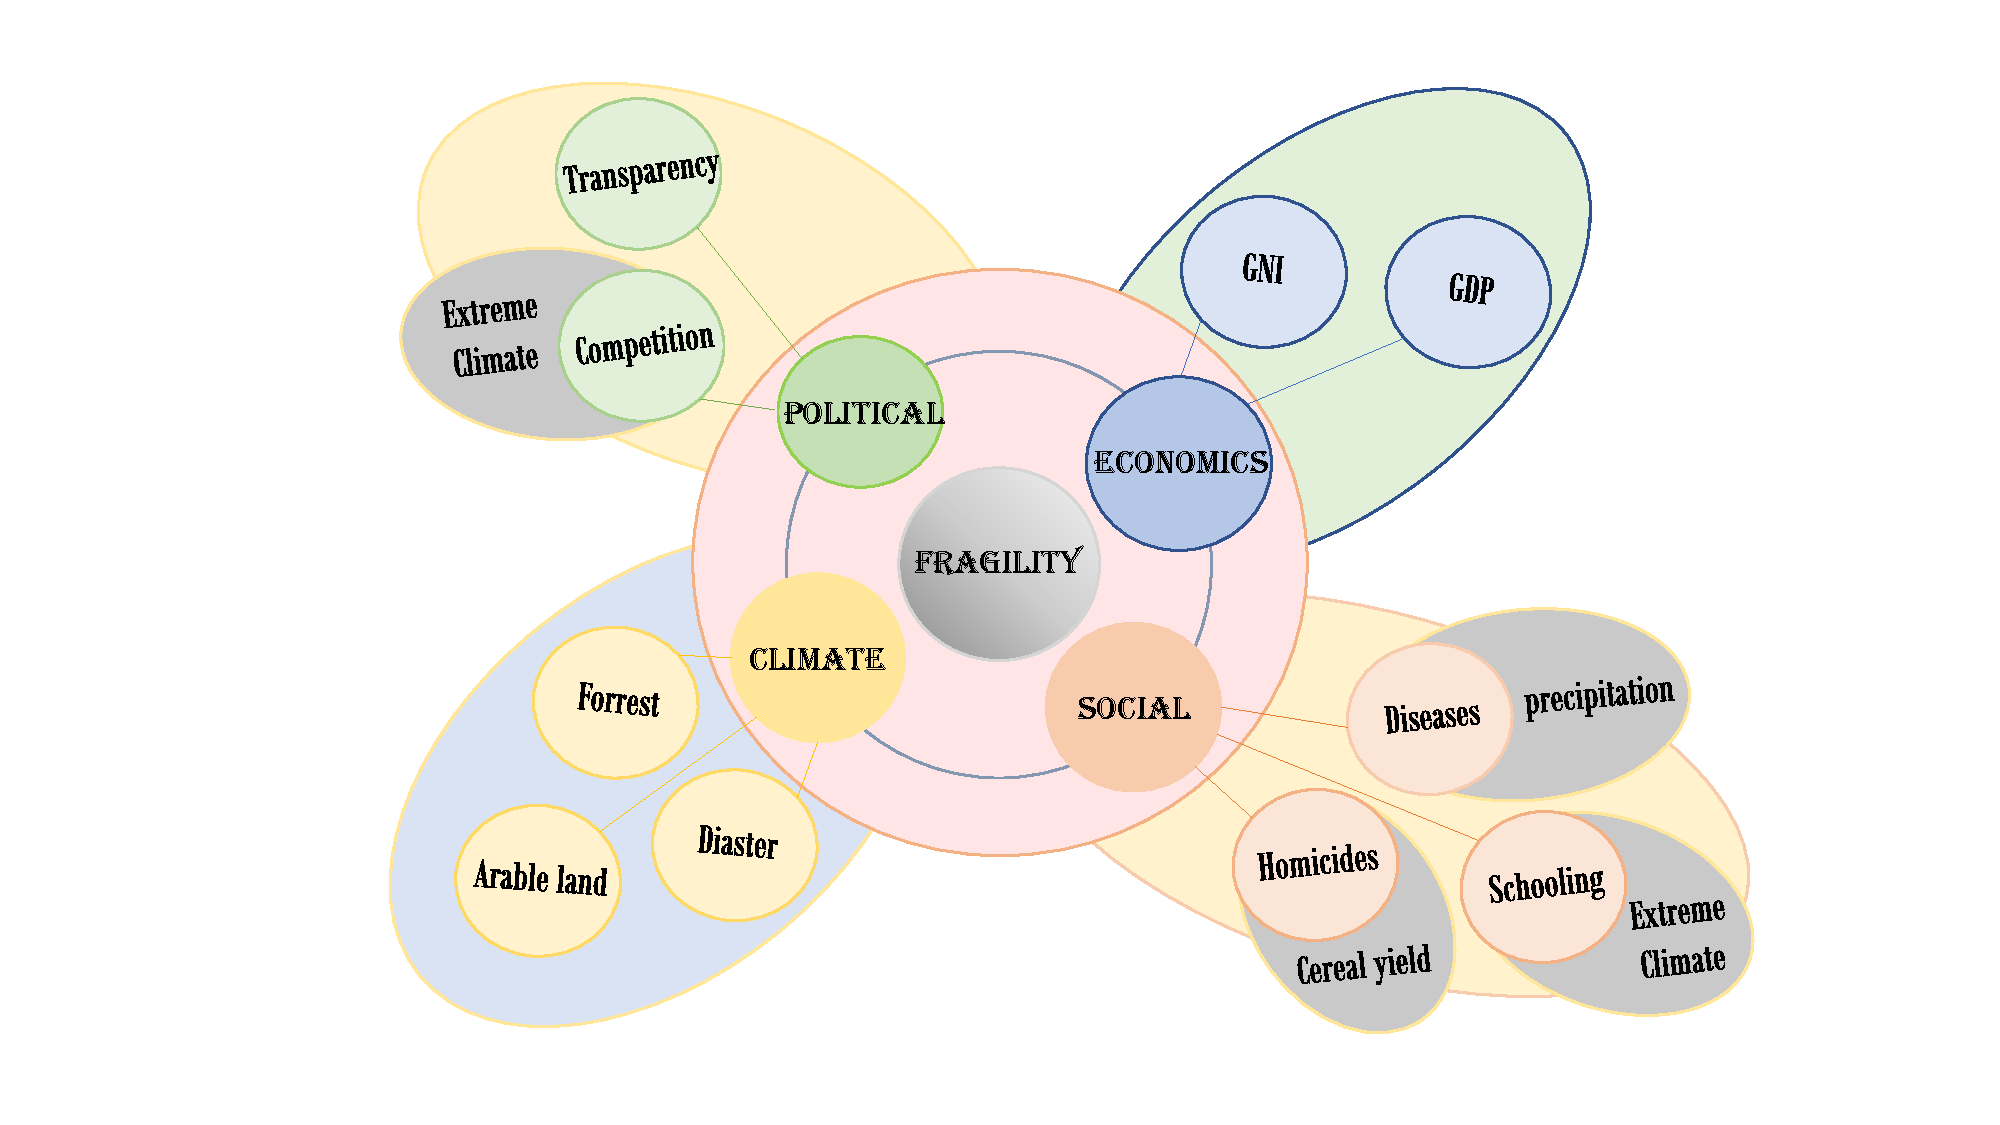
\includegraphics[width=15cm]{over-all-2.pdf}
			\caption{Process flow for the creation of the Fragility Index model. The model incorporated all ten indicators of smart growth and grouped them together into four principles. The sum of these metrics is the overall fragility Index.}
			\label{fig:over-all-2}
		\end{figure}
	
		
		 The establishment and solution of our models are as follow.
		
		
		\subsection{Primary Indicator System}
		
			\subsubsection{Select primary indicators by PCA}
		
				Fifty-six primary indicators are selected firstly to represent the regional fragility. Because there are plenty of signs is related, the method of PCA (Principal Component Analysis) is utilised to reduce the number of primary indicators. The selection of the indicators for fragility is based on four principles. 4 principles refer to ECONOMICS, SOCIETY, CLIMATE and POLITICS. The relationship between the indicators and the four principles should be that either the indicators can quantify the principles or principles that can dominate the changes in the indicators.
			
				The method of PCA is adopted to reduce the number of the indicator aforementioned. Eventually, 10 indicators are obtained. shown as in table \ref{fragility indicators}.
				
				\begin{table}[h]
					\caption{Framework of fragility indicators}
					\label{fragility indicators}
					\centering
					\begin{tabular}{p{3cm} p{7cm} p{4cm}}
						\specialrule{0.05em}{3pt}{3pt}
						Principles & Indicators &  Unit\\
						
						\specialrule{0.05em}{3pt}{3pt}
						\multirow{3}{*}{Climate} & Disaster & - \\
						\specialrule{0em}{3pt}{3pt}
						&Forest area& hectares per person \\
						\specialrule{0em}{3pt}{3pt}
						&  Arable land & percent \\
						
						\specialrule{0.05em}{3pt}{3pt}
						\multirow{2}{*}{Politics} & Political-competition &  -  \\
						\specialrule{0em}{3pt}{3pt}
						& Government transparency index &  -  \\
						
						\specialrule{0.05em}{3pt}{3pt}
						\multirow{3}{*}{Society} & Diseases &  percent \\
						\specialrule{0em}{3pt}{3pt}
						& Intentional homicides &  per 100,000 people \\
						\specialrule{0em}{3pt}{3pt}
						& Mean-years-of-schooling &  percent \\
						
						\specialrule{0.05em}{3pt}{3pt}
						\multirow{2}{*}{Economics} & GDP & current US\\
						\specialrule{0em}{3pt}{3pt}
						& GNI per capita & current internation\\
						\specialrule{0.05em}{3pt}{3pt}
						
					\end{tabular}
				\end{table} 
					
				
				
				The specific meaning of each indocator is listed in the table \ref{indicators} below.
				
				\begin{longtable}{p{4cm} p{10cm} }
					
					\caption{\label{indicators}Framework of fragility indicators}\\
					Indicator  & Explanation \\
					\noalign{\global\arrayrulewidth1pt}\hline\noalign{\global\arrayrulewidth0.4pt}
					Arable land & It represents synthetic action of precipitation and temperature variation\\
					Forest area  & It represents the size of forest cover\\
					Disaster & It represents the number of  disasters that have happened in current ten years \\
					Government transparency index& It represents the degree of government transparency\\
					Political-competition & It represents the degree of political competition\\
					GDP  & It represents the sum of the total value of the final products and services produced over a given period of time by all resident units in a country.\\
					GNI per capita  & It represents total value of goods and services produced over a period of time by all citizens of that country who have the nationality of that country\\
					Intentional homicides  & It represents the rate of intentional homicides happened per 100,000 people\\
					Diseases & It represents the degree of death caused by non-communicable diseases \\
					Mean years of schooling & It represents the average annual enrolment rate \\
					\hline
				\end{longtable}
				
			
			\subsubsection{Data normalization and conversion}
				
				Because the background of the 10 factors is different, the mechanism inside of them is complex, so it cannot be generalised directly. We first normalise the data between 0 and 1. Then we divide the factors into three categories, namely Cost-type class, Positive-type class and Specific-value class. The Cost-type category is that the larger the index value, the more vulnerable the region. The Positive-type class and the Cost-type class measure the opposite of the vulnerability. Specific-value Index affects a class that has an optimal value, and the degree of deviation from this value affects vulnerability.
				
				\begin{itemize}
					
					\item \textbf{Cost-type Index}
					
					\begin{equation}
					x = \frac{x -  x_{min}}{x_{max} -  x_{min}}
					\end{equation}
					
					where $x_{max} = max\{x_1, X_2, ... ,x_j\}$, $x_{min} = max\{x_1, X_2, ... ,x_j\}$. And $j$ is the number of countries.
					
					\item \textbf{Positive-type Index}
					
					\begin{equation}
					x = \frac{x_{max} - x}{x_{max} -  x_{min}}
					\end{equation}
					
					\item \textbf{Specific-value Index}
					
					\begin{equation}
					x = \frac{\vert q - x\vert}{x_{max} -  x_{min}}
					\end{equation}
					
					where $q$ is the best value of the indicator.
					
				\end{itemize}
			
			\subsubsection{Weighting Model Based on Entropy Weight Method(EWM)}
			
			Weighting models are required to evaluate the different contribution of the indicators. To get appropriate weight, Entropy Weight Method is chosen to calculate the weight vector in this section.
			
			We have already get $k$ indicators through PCA. These $k$ indicators are $X_1 \ldots X_K$ , and $X_i={x_1 \ldots x_n}$. Assume that the standardized values for each indicator data are $Y_1 \ldots Y_K$ ,So
			
			\begin{equation}
			Y _ { i j } = \frac { X _ { i j } - \min \left( X _ { i } \right) } { \max \left( X _ { i } \right) - \min \left( X _ { i } \right) }
			\end{equation}
			
			Let $P_{ij}$ denote the ratio of each indicator, it can be calculated by the following formula;
			
			
			\begin{equation}
				P _ { i j } = \frac { X _ { i j } } { \sum _ { j = 1 } ^ { m } X _ { i j } }
			\end{equation}
			
			Where the entropy value $e_i$ is obtained by the following formula:
			
			\begin{equation}
				e _ { i } = - k \sum _ { j = 1 } ^ { m } p _ { i j } \ln p _ { i j }
			\end{equation}
			
			According to the calculation formula of information entropy, the information entropy of each index is calculated as follows:$E_1 \ldots E_K$. 
			
			Calculating the weights of each index by information entropy as follows:
			
			
			\begin{equation}
				W _ { i } = \frac { 1 - E _ { i } } { k - \sum E _ { i } }
			\end{equation}
			
			According to the optimization model aforementioned, we can get the final weight. Since the correlation entropy is proportional to the weight, the final determined weight has a good positive correlation with the entropy in the modified optimization model.
			The specific indicator weight based on the data will be presented in Section 3.3.
		
									
			
		\subsection{Multiplier System}
		
			Even though we have outlined the basic structure of the model, we can see that climate change has a direct impact on vulnerability, but this model does not adequately reflect the full effect of climate on fragility.
		
			The links between climate change, conflict and fragility are not simple and linear. The increasing impacts of climate change do not automatically lead to more fragility and conflict. Rather, climate change acts as a threat multiplier. It interacts and converges with other existing risks and pressures in a given context and can increase the likelihood of fragility or violent conflict.
			
			Based on this, we propose a multiplier model to simulate the indirect and implicit climate-impact effects of climate change by affecting other indicators.
			
			We consider four climate change factors as potential indirect factors, and carefully analyze whether these four factors in combination with the indicator will affect the principals the indicator belong to. Four climate change refers to Arable Land (hectares per person), Number of Natural Disaster in Recent Ten Years, Temperature and Humidity.
			
			\subsubsection{Select Implicit Impact Pattern}
			
				We divide each potential indicator into three classes and observe the difference between the three sets of data. The more significant difference has, the greater impact the potential indicator has. Based on this, we define a metric to measure the impact of potential indicators:
				
				Let i denote the i-th potential indicators and j denote j-th indicators.
				
				\begin{equation}
				M_{ij} = \sqrt{\frac{1}{N}\sum_{k=1}^N (x_i - x_i^{mean})^2}
				\end{equation}
				
			\subsubsection{Determine Multiplier}
			
				We believe that climate factors act as a multiplier on the indicator and further affect regional instability. This multiplier is not constant, but changes with climatic factors.
			
				We have investigated the pattern where climate and indicators interact, so quantifying the impact of climate on principle through indicators is a must.
				
				In different climatic conditions, if the relationship between the principle and the indicator changes, this indicates that the weather has an indirect effect.
				
				Let's take one of the patterns as an example. When the Average Precipitation Depth(multiplier) is not considered, the relationship between the Intentional homicide rate(indicator) and the Society(principal) is:
				
				\begin{equation}
				\mathrm { P_{Society} } = f \left( \text {indicator} _ { homicide } \right)
				\end{equation}
				
				Where:
				$P_{Society}$ represent the Social Instability.\\
				$indicator_ { homicide }$ denotes Intentional homicide rate.
				
				
				And then we take Average Precipitation Depth(multiplier) into consideration:
				
				\begin{equation}
				\mathrm { P_{Society} } = f \left( \text {indicator} _ { homicide } , w _ { precipitation } \right)
				\end{equation}
				
				Where $w _ { precipitation }$ represent Average Precipitation Depth.
				
				And finally we can difine the Multipler effect of Pattern Precipitation-Homicide-Society:
				
				\begin{equation}
				Multiplier_{ij} = \frac { \partial f \left( \text {indicator} _ { j } \right) } { \partial \text {  indicator } _ { j } } / \frac { \partial f \left( \text {indicator} _ { j } , w _ { i } \right) }  { \partial \text {  indicator } _ { j } }
				\end{equation}
				
				
				\subsubsection{Multiplier System}
				
					We divide the indirect effects of climate into four situations.
					
					\begin{itemize}
						
						\item \textbf{No impact at all.} \\In this case the role of the indicator is completely unaffected by climatic conditions. Reflected in the figure below, the slopes of the three straight lines are basically the same, indicating that the indicators have the same effect on the index under different climatic conditions.
						
						\begin{figure}[h]
							\small
							\centering
							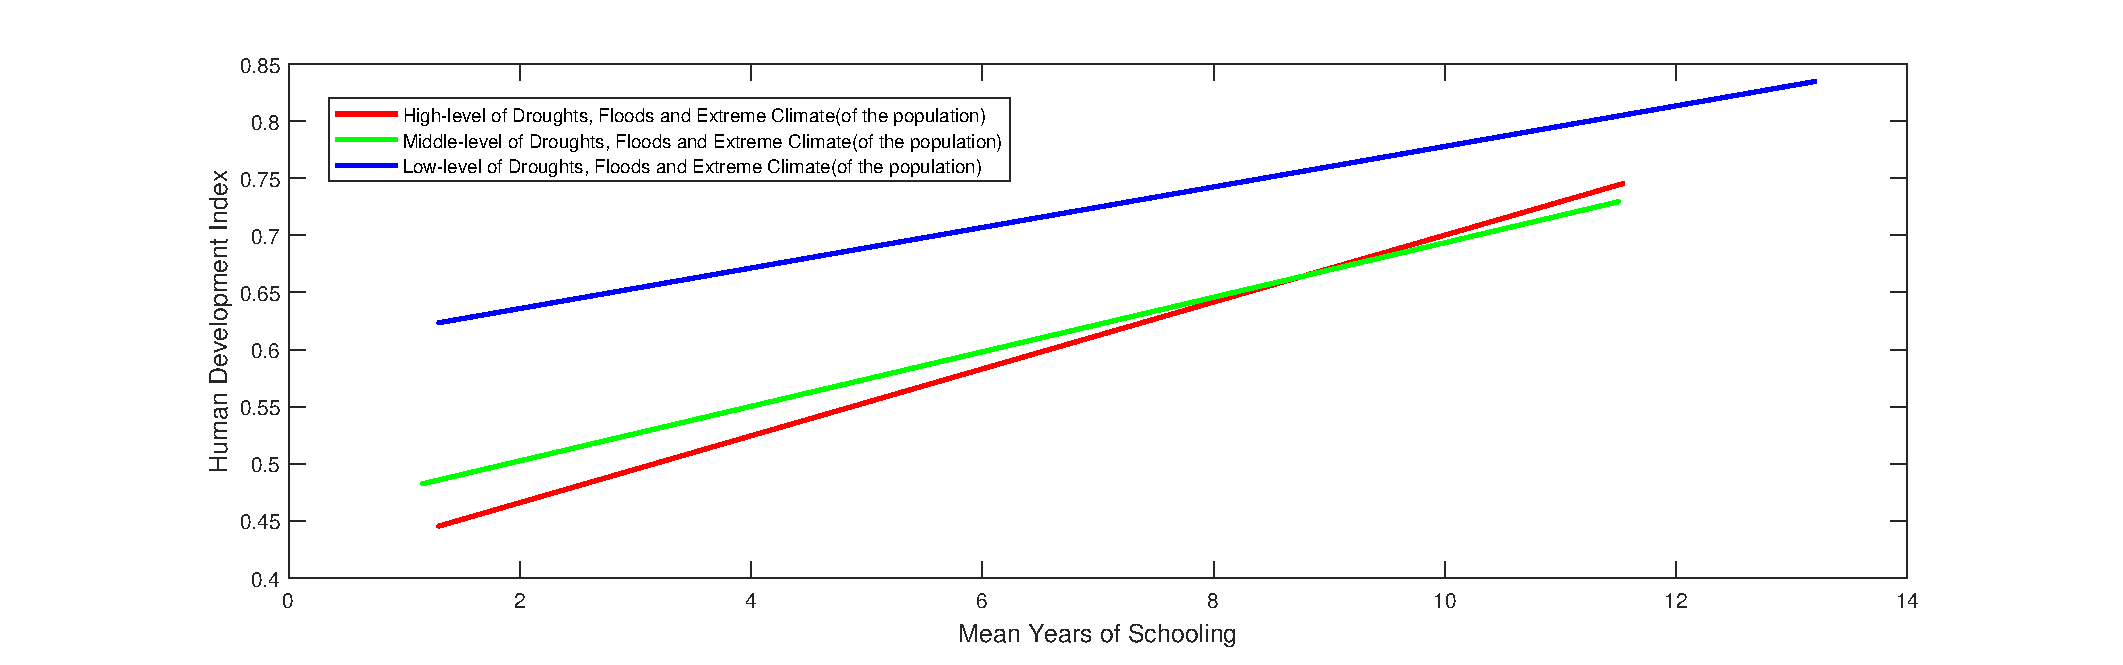
\includegraphics[width=14cm]{multiplier-4.eps}
							\caption{The Multiplier Effect Pattern-1}
							\label{fig:multiplier-4}
						\end{figure}
						
						\item \textbf{Positive or negative correlation.}\\ As the climate changes, the role of indicators is also growing. As shown in the figure below, the slope between the three fitted changes with the change of the climatic state, and the slope from the red line to the blue line increases sequentially, indicating that the influence of the indicator on the index under different climatic conditions is affected by the climate. To the effect, the higher the climate state value, the stronger the role of the indicator.
						
						\begin{figure}[h]
							\small
							\centering
							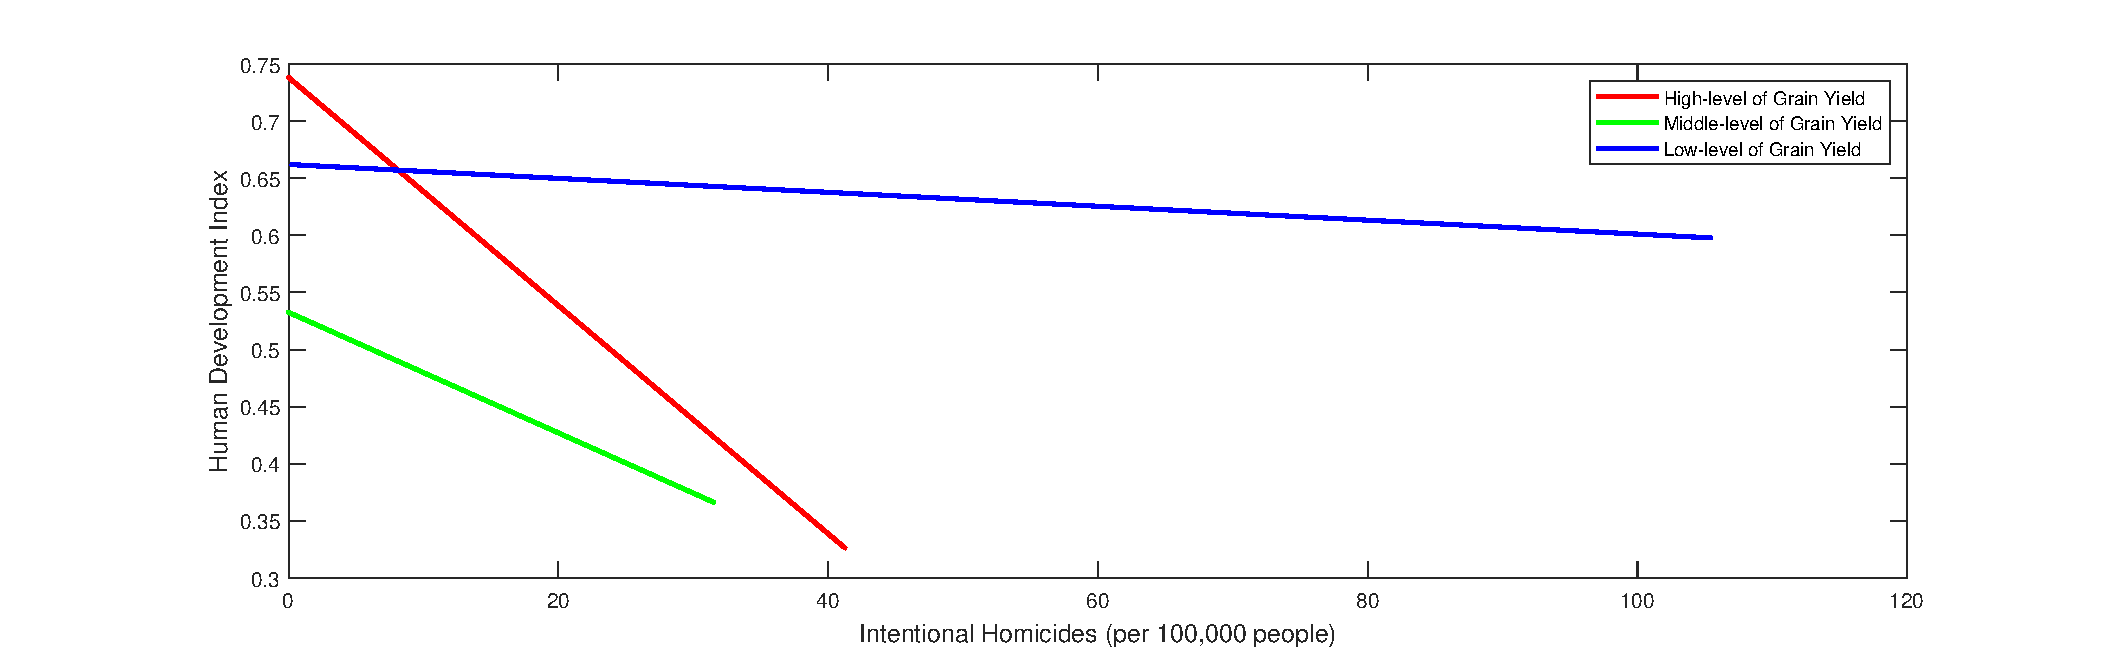
\includegraphics[width=14cm]{multiplier-2.eps}
							\caption{The Multiplier Effect Pattern-2}
							\label{fig:multiplier-2}
						\end{figure}
						
						
						\item \textbf{Threshold impact.}\\ There is a threshold, and when the climate change reaches the threshold, it will affect the indicator. There is no impact before the threshold is reached. As shown in the figure below, the slopes of the three lines fitted, the slopes of the red and green lines did not change significantly, and the slope of the blue line changed significantly, indicating that there is a threshold. The state of the climate does not affect the action of the indicator until the climate state value reaches this threshold, and the state of the climate begins to affect the role of the indicator after the threshold is reached. 
						
						\begin{figure}[h]
							\small
							\centering
							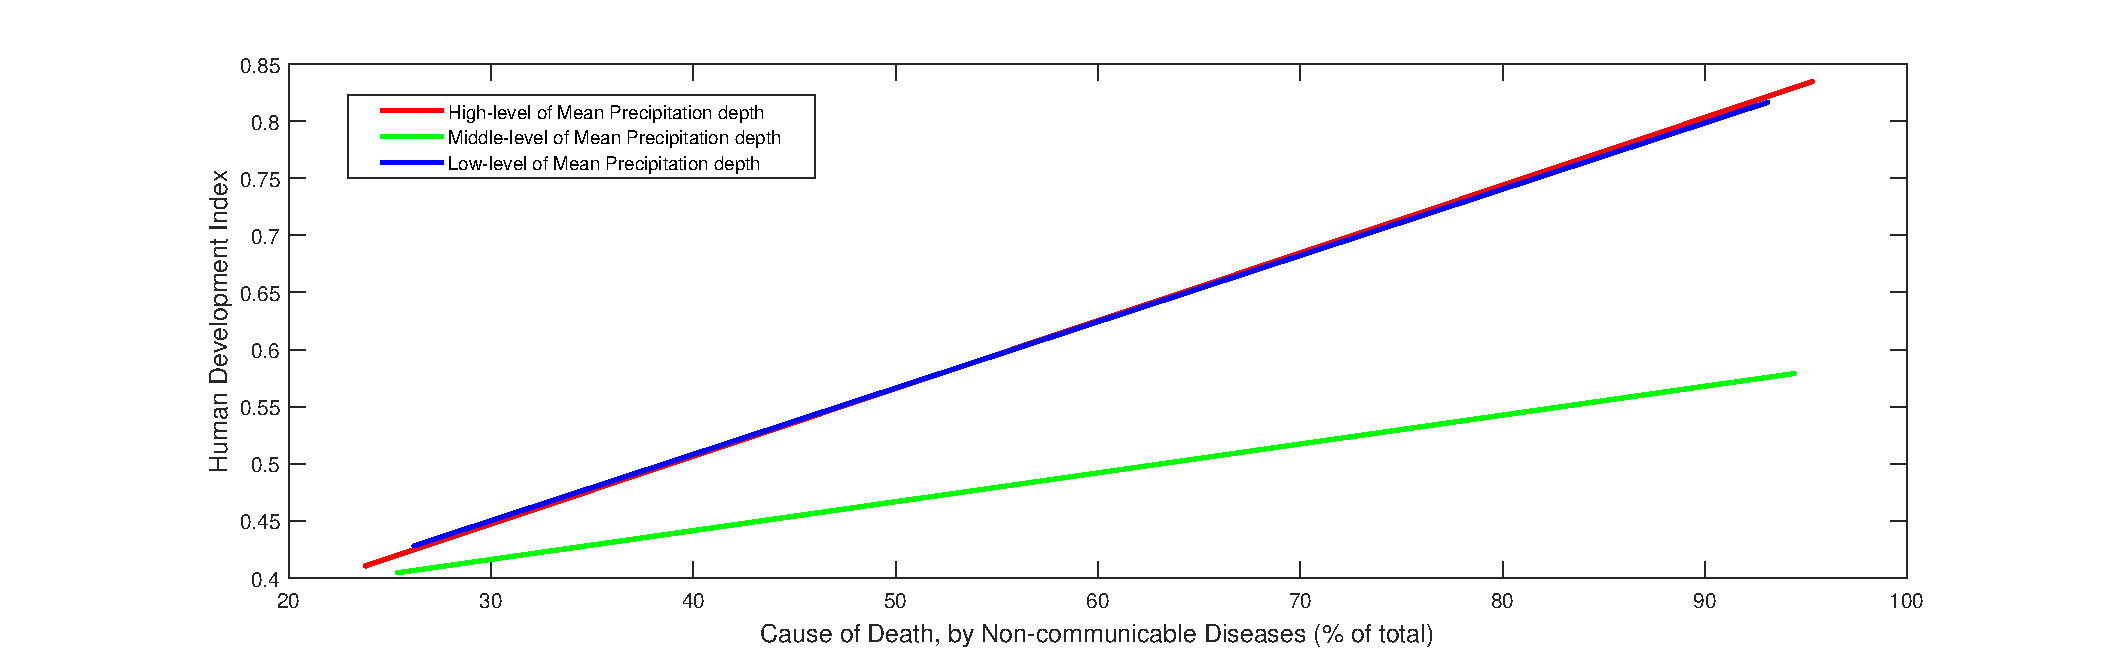
\includegraphics[width=14cm]{multiplier-1.eps}
							\caption{The Multiplier Effect Pattern-3}
							\label{fig:multiplier-1}
						\end{figure}
						
						\item \textbf{The optimal value impact.} \\there is an optimal value for the state value of the climate, and the state value of the climate is closer to the optimal value. Then, the greater his influence on the role of the indicator, the more he deviates from the optimal value, the smaller his influence.
						
						\begin{figure}[h]
							\small
							\centering
							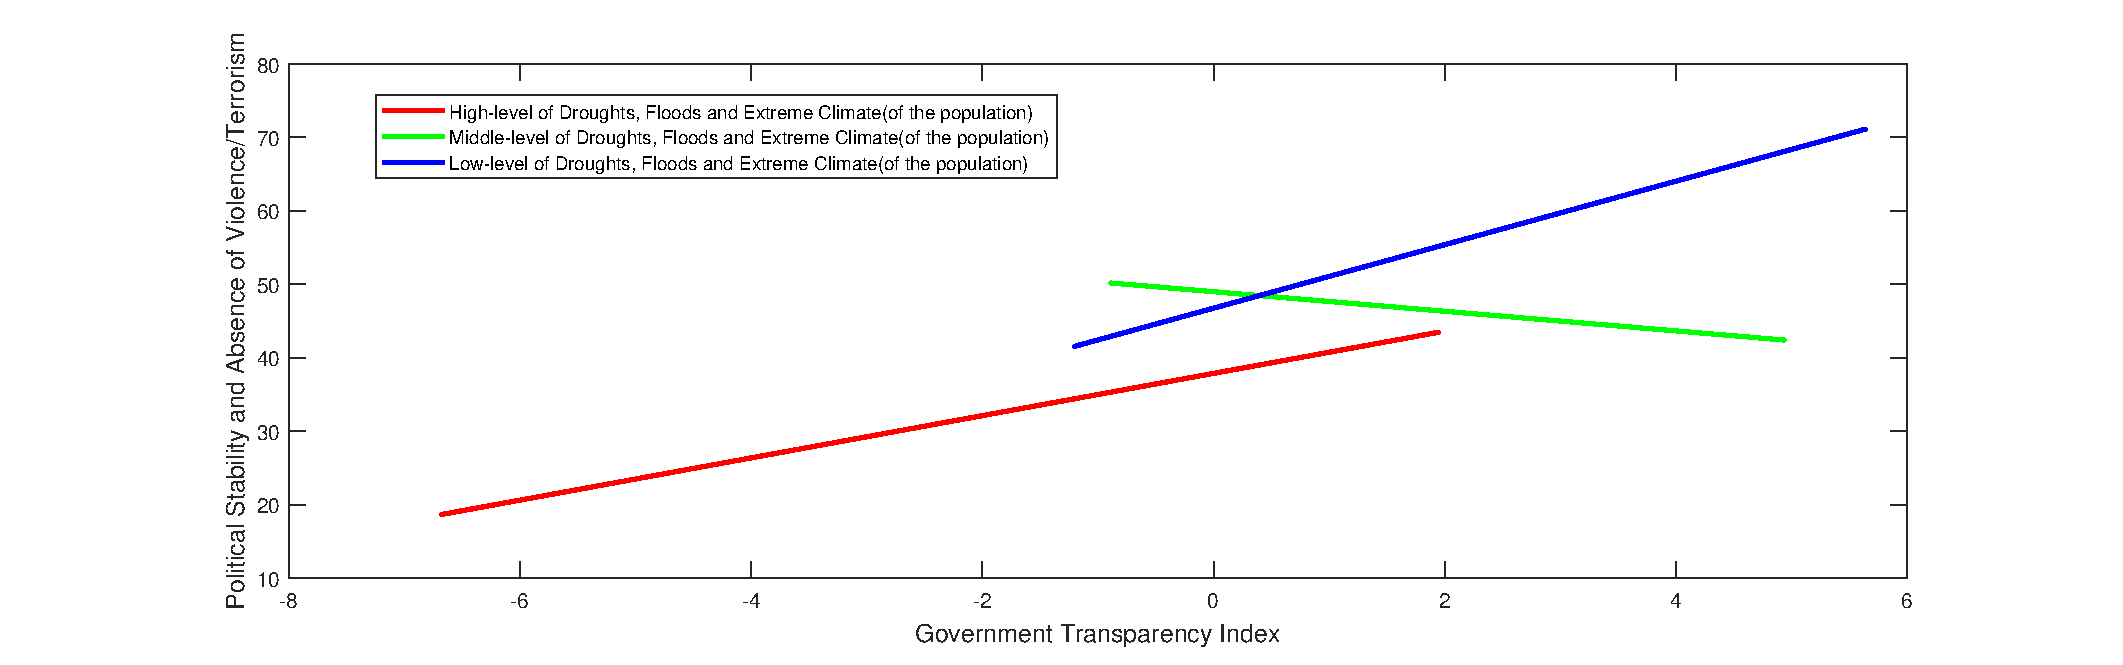
\includegraphics[width=14cm]{multiplier-3.eps}
							\caption{The Multiplier Effect Pattern-4}
							\label{fig:multiplier-3}
						\end{figure}
						
					\end{itemize}
				
					Through analysis, the patterns we get that indicators are affected by climate change are below:
					
					\begin{table}[h]
						\caption{Framework of fragility indicators}
						\label{fragility-indicators}
						\centering
						\renewcommand\arraystretch{1.32}
						\begin{tabular}{p{6cm}p{6cm}c}
							\hline
							Climate & Indicator & Principle\\
							\noalign{\global\arrayrulewidth1pt}\hline\noalign{\global\arrayrulewidth0.4pt}
							Average precipitation depth & Diseases & Society\\
							Cereal production & Intentional homicides & Society\\
							Extreme temperatures & Government-transparency-index & Politics\\
							Extreme temperatures & Political-competition & Society\\
							\hline
						\end{tabular}
					\end{table} 
				
			
		\subsection{Comprehensive Evaluation Index}
		
			\subsubsection{Determination of indicator index}
		
				Four principles are identified after selecting a set of comprehensive and effective primary indicators and determining the reasonable weights, including The Society, Climate, Politics and Economics. Notably, these four principles will be used to evaluate the four dimensions of the fragility.
				
				\begin{figure}[h]
					\small
					\centering
					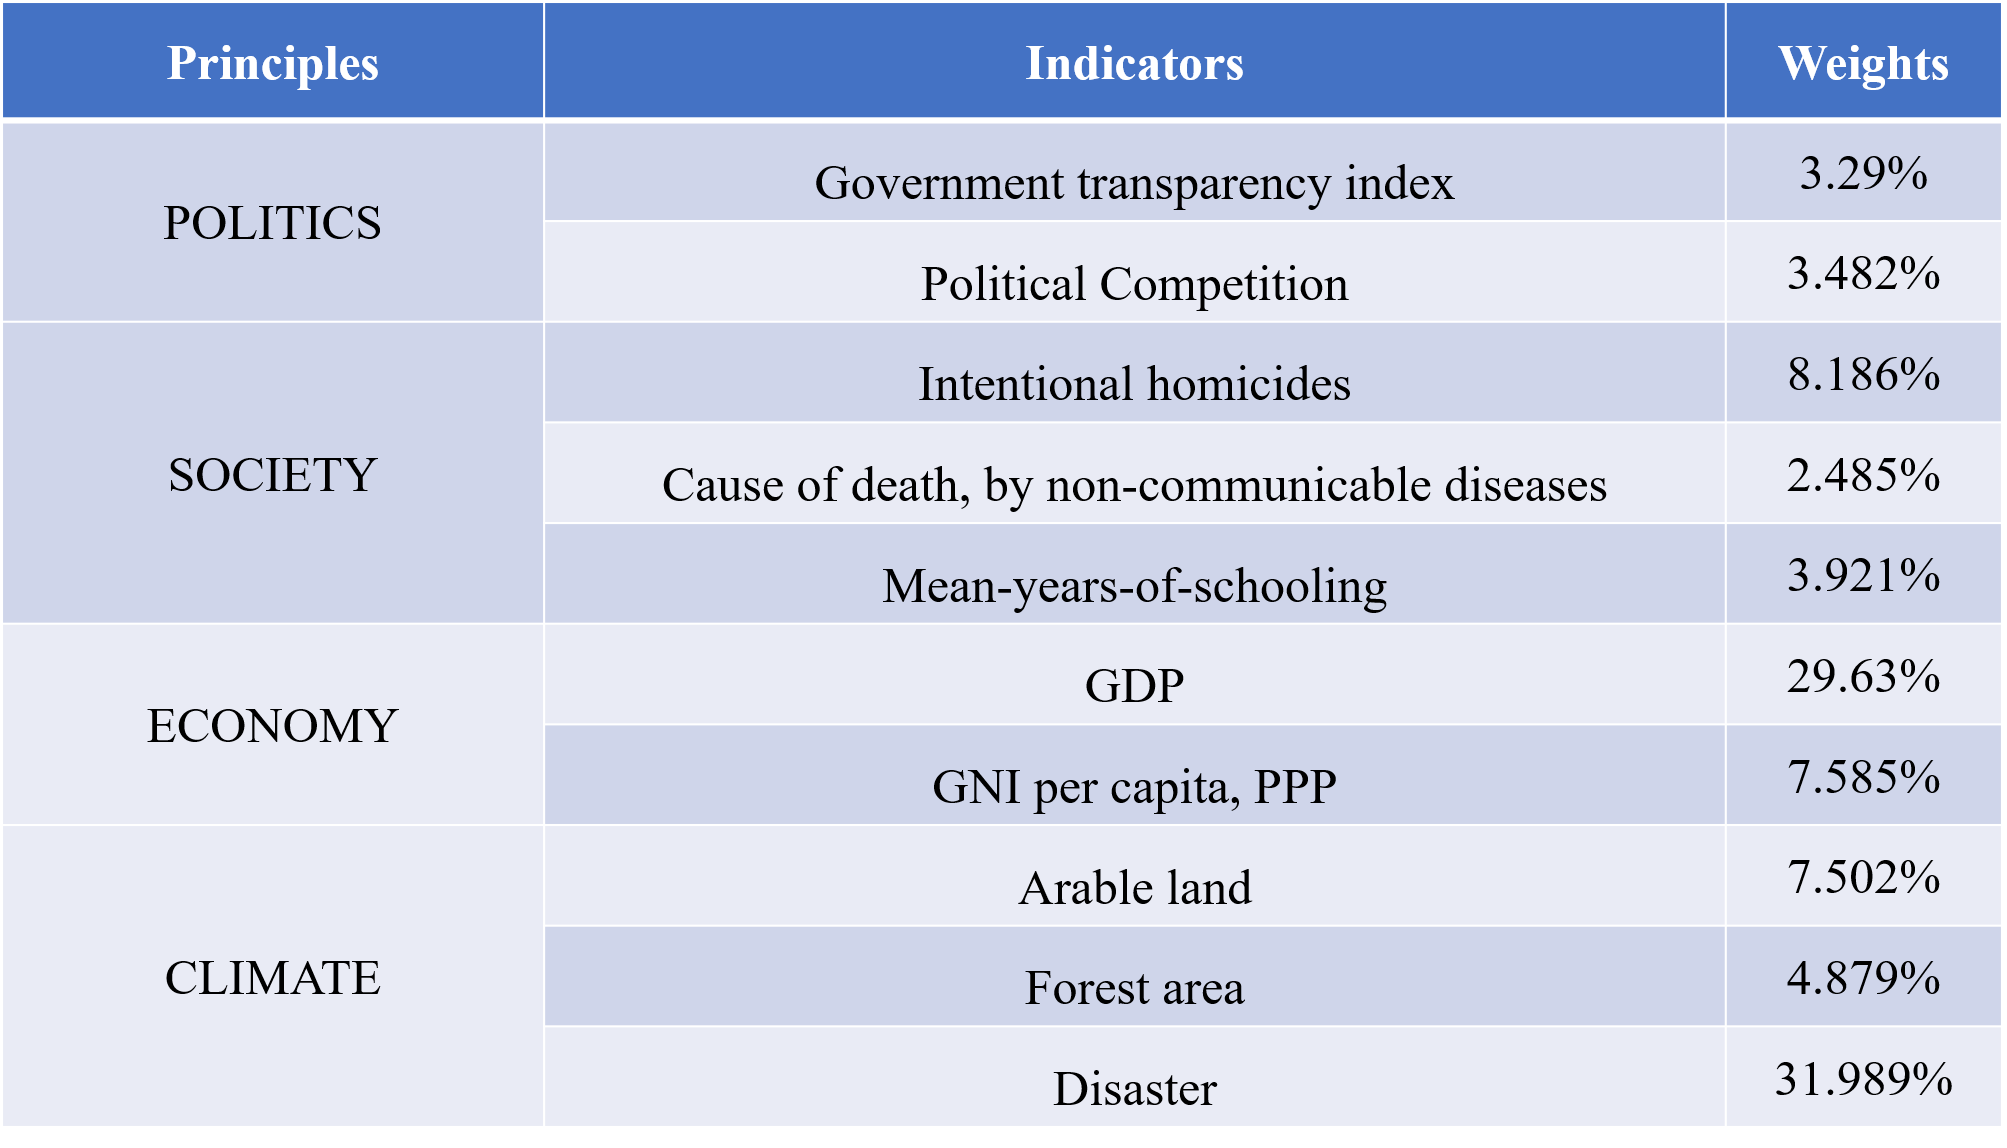
\includegraphics[width=14cm]{weights.png}
					\caption{The Weight of Indicators}
					\label{fig:weights}
				\end{figure}
				
				Economics is the most important index of smart growth. Economics mainly contains two indicators. It’s primarily used to reflect the efficiency of economics using,
				the diversity of the market and the rationality of economic planning, etc.
				
				Society considers the gap between the rich and poor, the protection of socially vulnerable groups (e.g. women, children, the poor). Moreover, it also takes safety into account.
				
				Politics includes the efficiency of government work, the impact of political struggle on the state, and of course the degree of political corruption in a country is also taken into account.
				
				The climate is mainly affected by geographical location, which has long influenced the grain output of a country and can reflect the stability of a state to some extent.
			
				
			
			\subsubsection{Determination of multiplier system}
			
				Through analysis, we have four indicators that will be affected by climate change, let us use $\beta_{j}$ to represent multiplier affected on j-th indicator.
				
				$$ 
				\beta_{j}=\left\{
				\begin{array}{rcl}
				Multiplier_{j}       &      & if \ indicator_{j} \ is \ affected \ by \ climate \\
				1     &      & if \ indicator_{j} \ is \ not \ affected \ by \ climate\\
				\end{array} \right. 
				$$ 
				
				The final Fragility calculation formula is as follows:
				
				\begin{equation}
					Fragility =  Politics + Climate + Economy + Society
				\end{equation}
				
				and
				
				$$ 
				\beta_{j}=\left\{
				\begin{array}{rcl}
				Climate& =& \alpha _ { 1 } A L + \alpha _ { 2 } F A + \alpha _ { 3 } D I\\
				Politics& =& \alpha _ { 4 } \beta _ { 4 } G T I + \alpha _ { 5 } \beta _ { 5 } P L C\\
				Economics& =& \alpha _ { 6 } \beta _ { 6 } G D P + \alpha _ { 7 } \beta _ { 7 } G N\\
				Society& =& \alpha _ { 8 } \beta _ { 8 } I H + \alpha _ { 9 } \beta _ { 9 } D C B N + \alpha _ { 10 } \beta _ { 0 } M T O S
				\end{array} \right. 
				$$
				
				Based on our model, we calculated the 264 countries in the world and derived the following rankings:
				
				\begin{figure}[h]
					\small
					\centering
					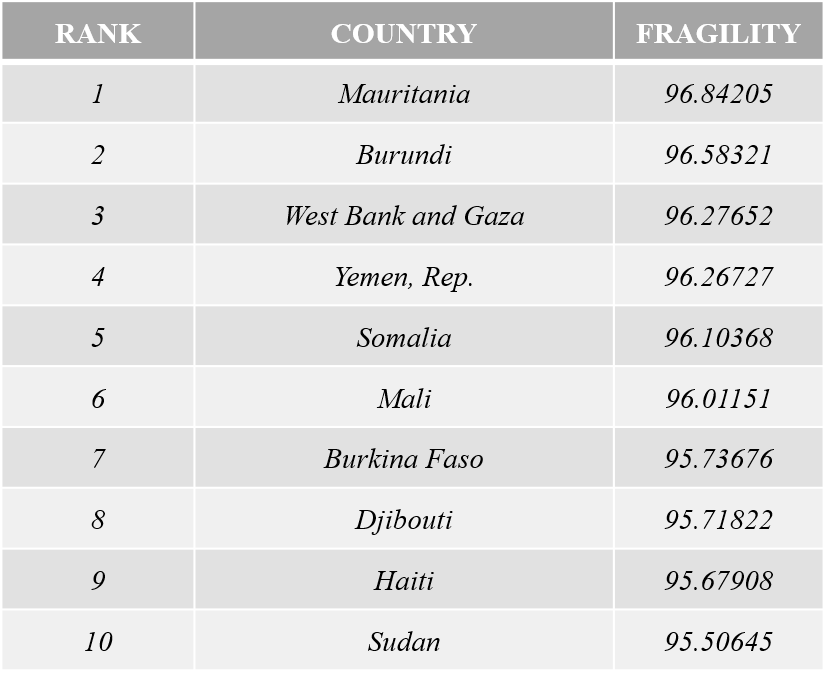
\includegraphics[width=10cm]{rank.png}
					\caption{The Top-10 Countries in the rank}
					\label{rank}
				\end{figure}
				
		
		\subsection{Three-levels Evaluation}
		
			\subsubsection{Standard Setting Based on CFSFDP}
		
				Although a continuous index evaluation has been established aforementioned, a suitable standard is still needed to assess the regional is fragile, vulnerable or stable. Consequently, CFSFDP (Clustering by fast search and find of density peaks) is adapted to make a reasonable standard.
				
				For each data point $i$, we compute two quantities: its local density $r_i$ and its distance $d_i$ from points of higher density. Both these quantities depend only on the distances $d_ij$ between data points, which are assumed to satisfy the triangular inequality. The local density $r_i$ of data point i is defined as:
				
				\begin{equation}
				\rho _ { i } = \sum _ { j } \chi \left( d _ { i j } - d _ { \mathrm { c } } \right)
				\end{equation}
				
				where $\chi ( x ) = 1$ if $ x < 1 $ and $\chi ( x ) = 0$ otherwise, and $d_c$ is a cutoff distance. 
				
				$d_i$ is measured by computing the minimum distance between the point $i$ and any other point with higher density:
				
				\begin{equation}
				\delta _ { i } = \min _ { j : \rho _ { j } > \rho _ { i } } \left( d _ { i j } \right)
				\end{equation}
				
				Those points with a large local density $\rho _ { i }$ and a large $delta _ { i }$ are considered to be the center of the cluster. The point where the local density is small but δi is large is the abnormal point.
				
				After the cluster center is determined, the remaining points are assigned to the same cluster as its nearest neighbor with a higher density.
				
				Once we have identified three clusters, then the mean of the boundary point of different clusters are used as the standard boundary.
			
			\subsubsection{The Standard of Regional Instability}
			
				The standard of Regional Instability is obtained eventually in this section, according to the CFSFDP mentioned above. 
				
				The reason why CFSFDP is chosen instead of using K-Means directly is:
				
				\begin{itemize}
					
					\item K-Means is very sensitive to the choice of the initial cluster center. When we cluster one-dimensional data, this sensitivity will increase further.
					
					\item K-means is greatly affected by the outliers. When the amount of data is not large, using K-Means will result in poor clustering.
					
				\end{itemize}
				
				
				So we finally chose to use CFSFDP instead of K-Means. We used the kernel density estimate to determine the initial cluster center:
				
				\begin{figure}[h]
					\small
					\centering
					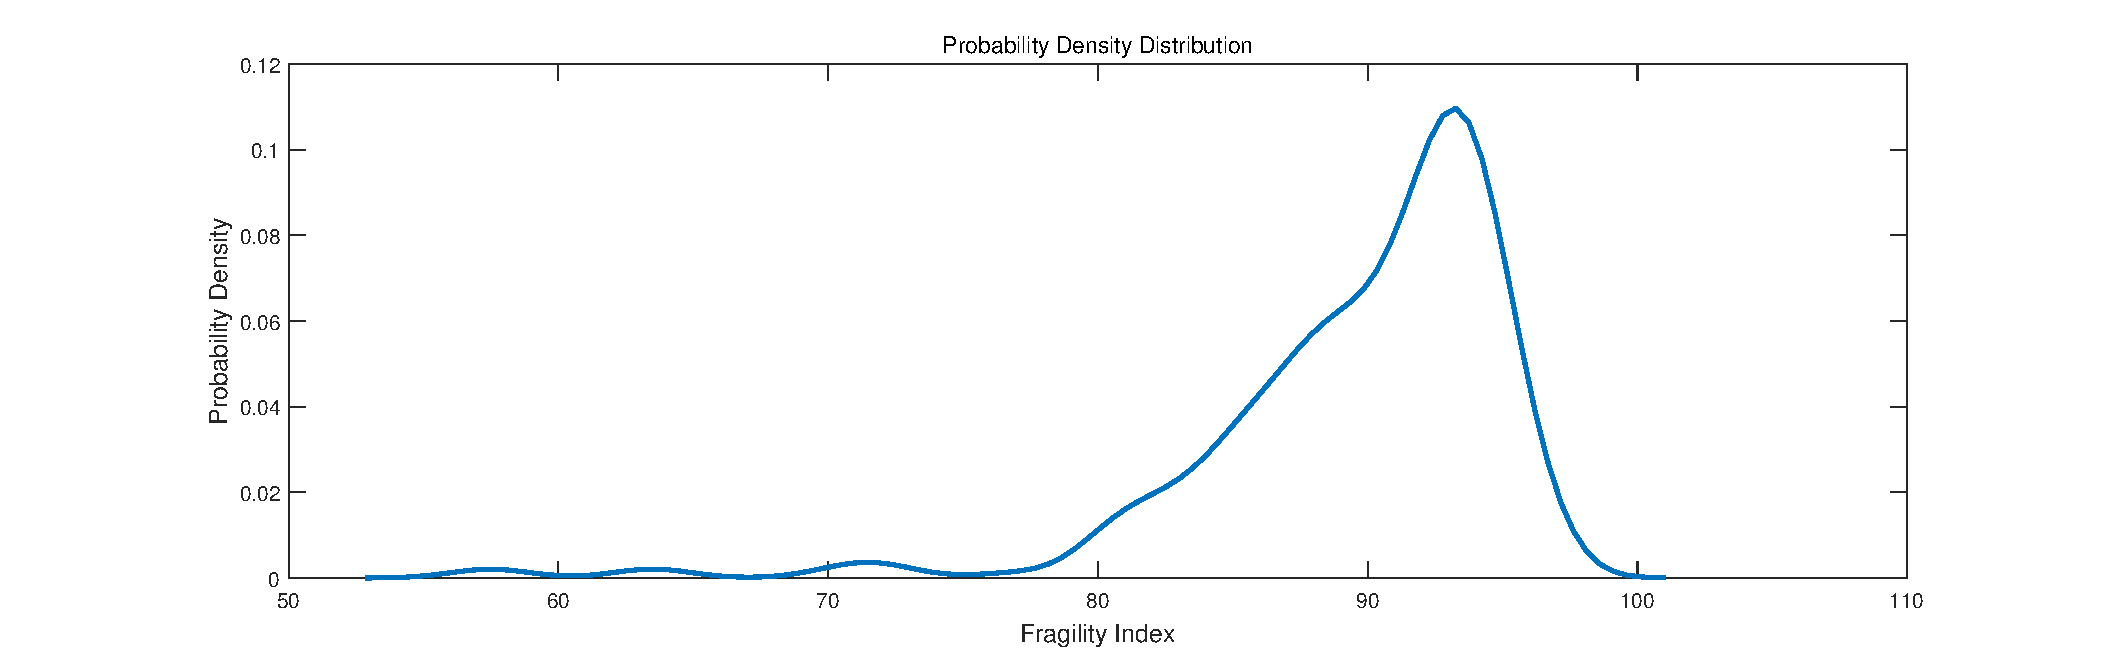
\includegraphics[width=14cm]{hemidu.eps}
					\caption{The Result of Kernel Density Estimation}
					\label{fig:hemidu}
				\end{figure}
				
				\clearpage
				
				Based on this, the remaining points are clustered using local density:
				
				\begin{figure}[h]
					\small
					\centering
					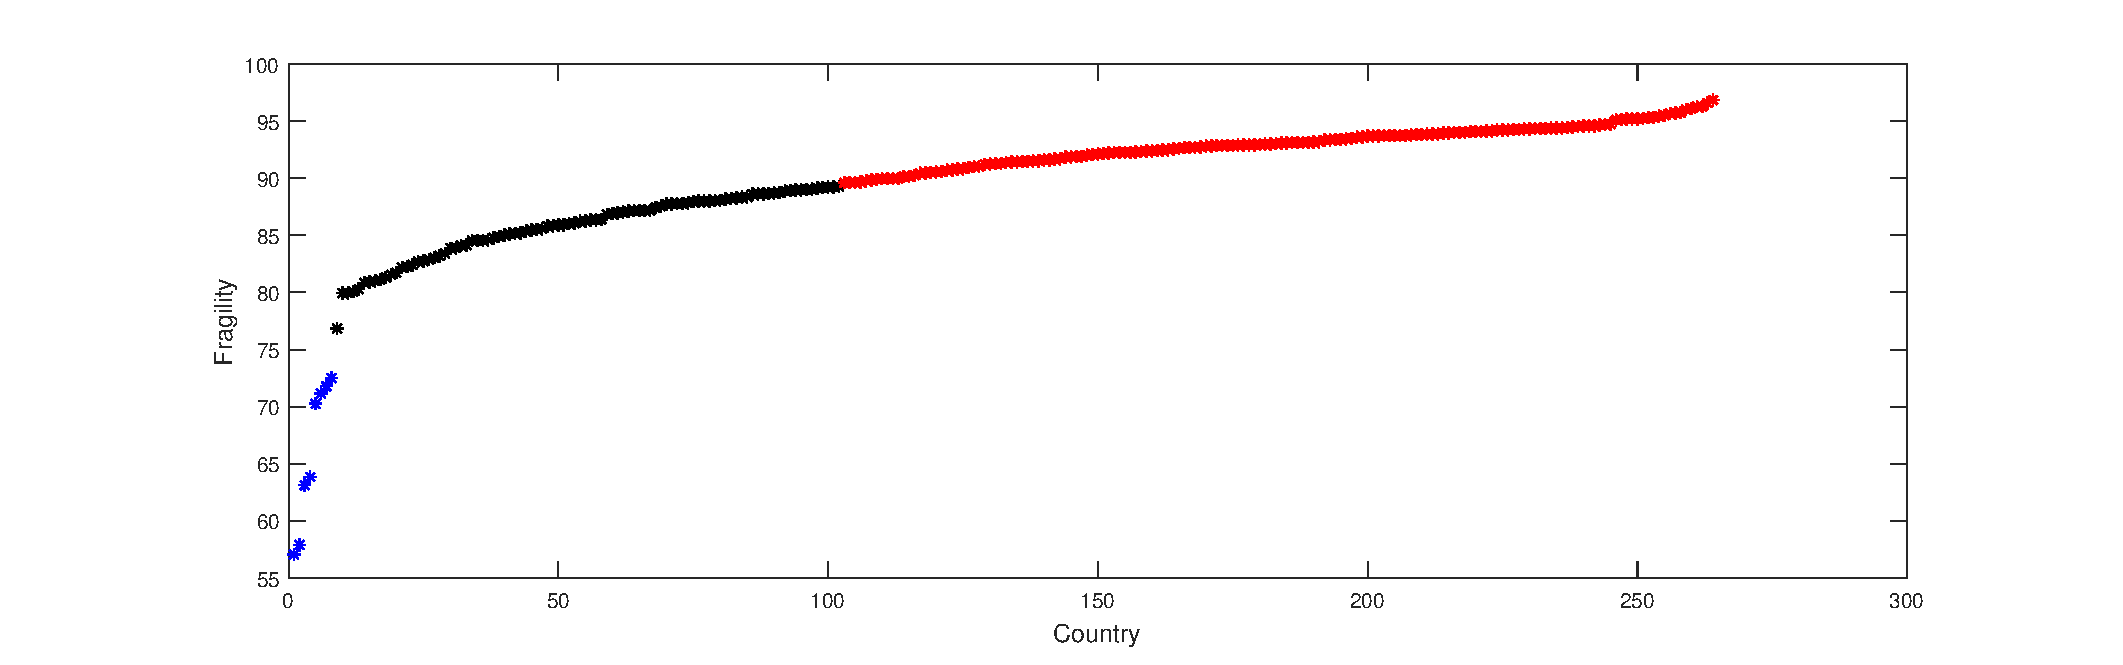
\includegraphics[width=14cm]{kmeans1.eps}
					\label{fig:kmeans1}
				\end{figure}
			
				\begin{figure}[h]
					\small
					\centering
					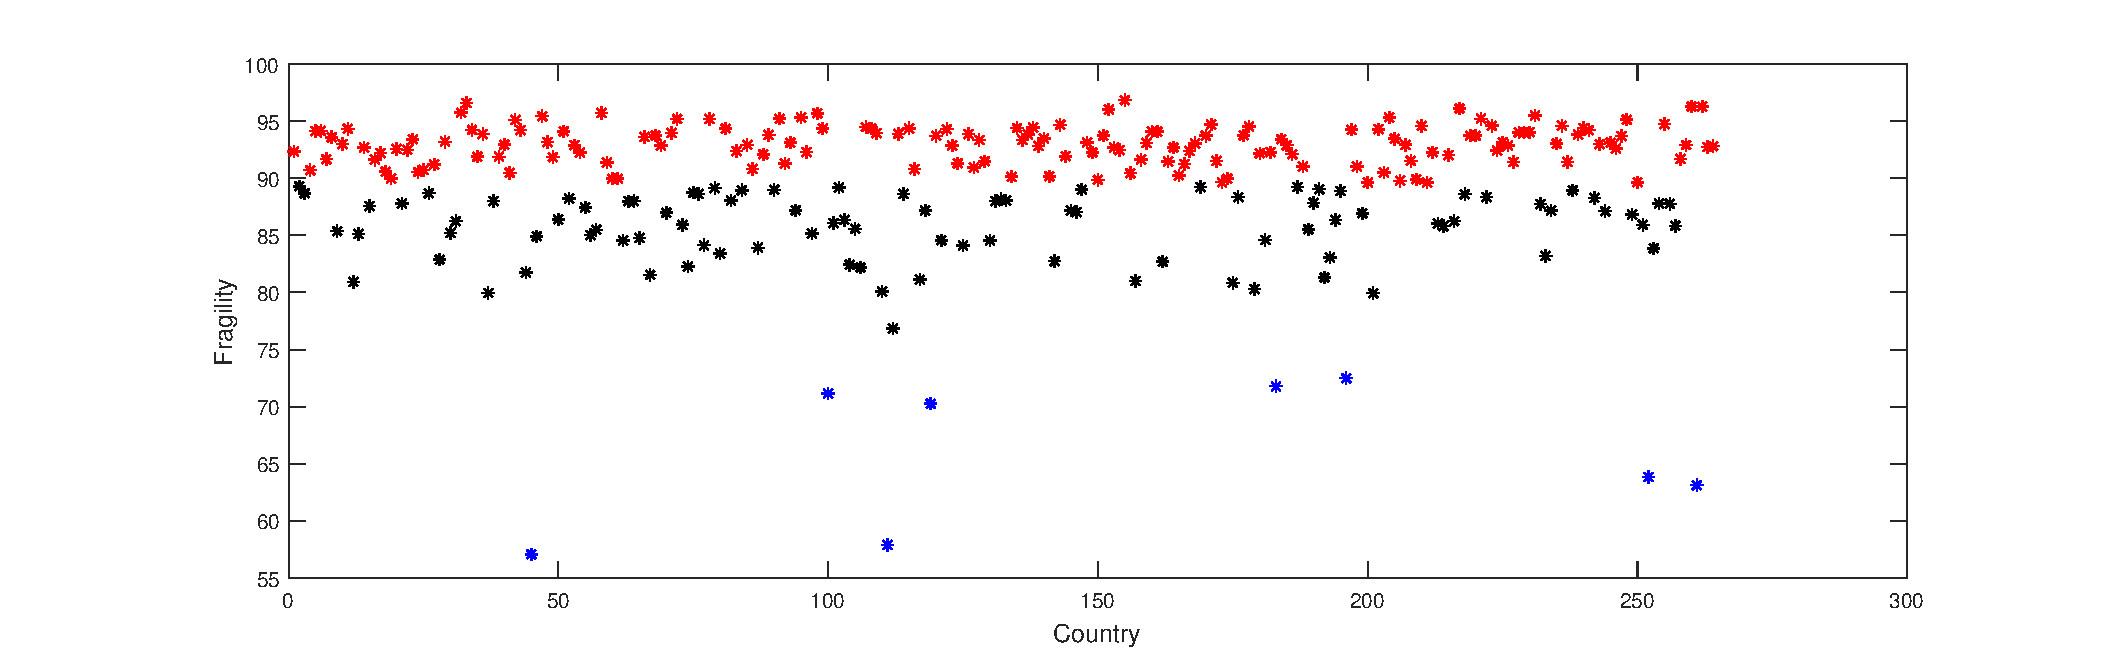
\includegraphics[width=14cm]{kmeans2.eps}
					\caption{The Result of CFSFDP}
					\label{fig:kmeans2}
				\end{figure}
				
				
				
				In the end, we can get two tipping points: 77 \& 89.5
				
				\begin{itemize}
					
					\item When a country’s fragility index exceeds 87.5, it indicates that the country is in a very instable state, we call them fragile region.
					
					\item When a country's fragility index is between 87.5 and 77, it indicates that the country is in a vilnerable state. At this time, climate change will affect the stability of the country, and the state can also reduce the risk of climate change through human intervention measures.
					
					\item When a country's fragility index is below 77, it indicates that the country is in a stable state, when climate change has little impact on the country.
					
				\end{itemize}
				
	
	\section{Anaylsis for Two Countries}
		\subsection{Anaylsis for Yemen}
			
			When measuring the impact of climate change,we can calculate the direct impact of climate change by calculating the change of these factors . We can calculate the indirect impact of climate change by calculating fragility change after subtracting 1 from its multiplier factor.
			Through our model, we calculate the whole impact of climate as follows:
			
			\begin{equation}
			Fragility =  Politics + Climate + Economy + Society
			\end{equation}
			
			$$ 
			\beta_{j}=\left\{
			\begin{array}{rcl}
			\Delta Climate& =& \alpha _ { 1 } A L + \alpha _ { 2 } F A + \alpha _ { 3 } D I\\
			\Delta Politics& =& \alpha _ { 4 } (1-\beta _ { 4 }) G T I + \alpha _ { 5 } \beta _ { 5 } P L C\\
			\Delta Economics& =& \alpha _ { 6 } (1-\beta _ { 6 }) G D P + \alpha _ { 7 } \beta _ { 7 } G N\\
			\Delta Society& =& \alpha _ { 8 } (\beta _ { 8 }) I H + \alpha _ { 9 } (\beta _ { 9 }) D C B N + \alpha _ { 10 } \beta _ { 0 } M T O S
			\end{array} \right. 
			$$
			
			In this paper , Yemen is selected as example to analyze the task 2. In our model , the fragility index of Yemen is 96.2673. The reason why we  choose Yemen is that it is in both our model’s top-10 and Fragile State Index’s top-10. We collect Yemen’s data through Worldbank’s website and Our world in data website.
			
			Through our model,we can get the magnitude of the climate change impact on each indicator. So we can get the difference in fragility before and after climate impacts. By calculation, we can show the country's fragility before and after removing climate impact in the chart below.
			
			\begin{figure}[htbp]
				\centering
				\subfigure[Before]{
					\begin{minipage}[t]{0.5\linewidth}
						\centering
						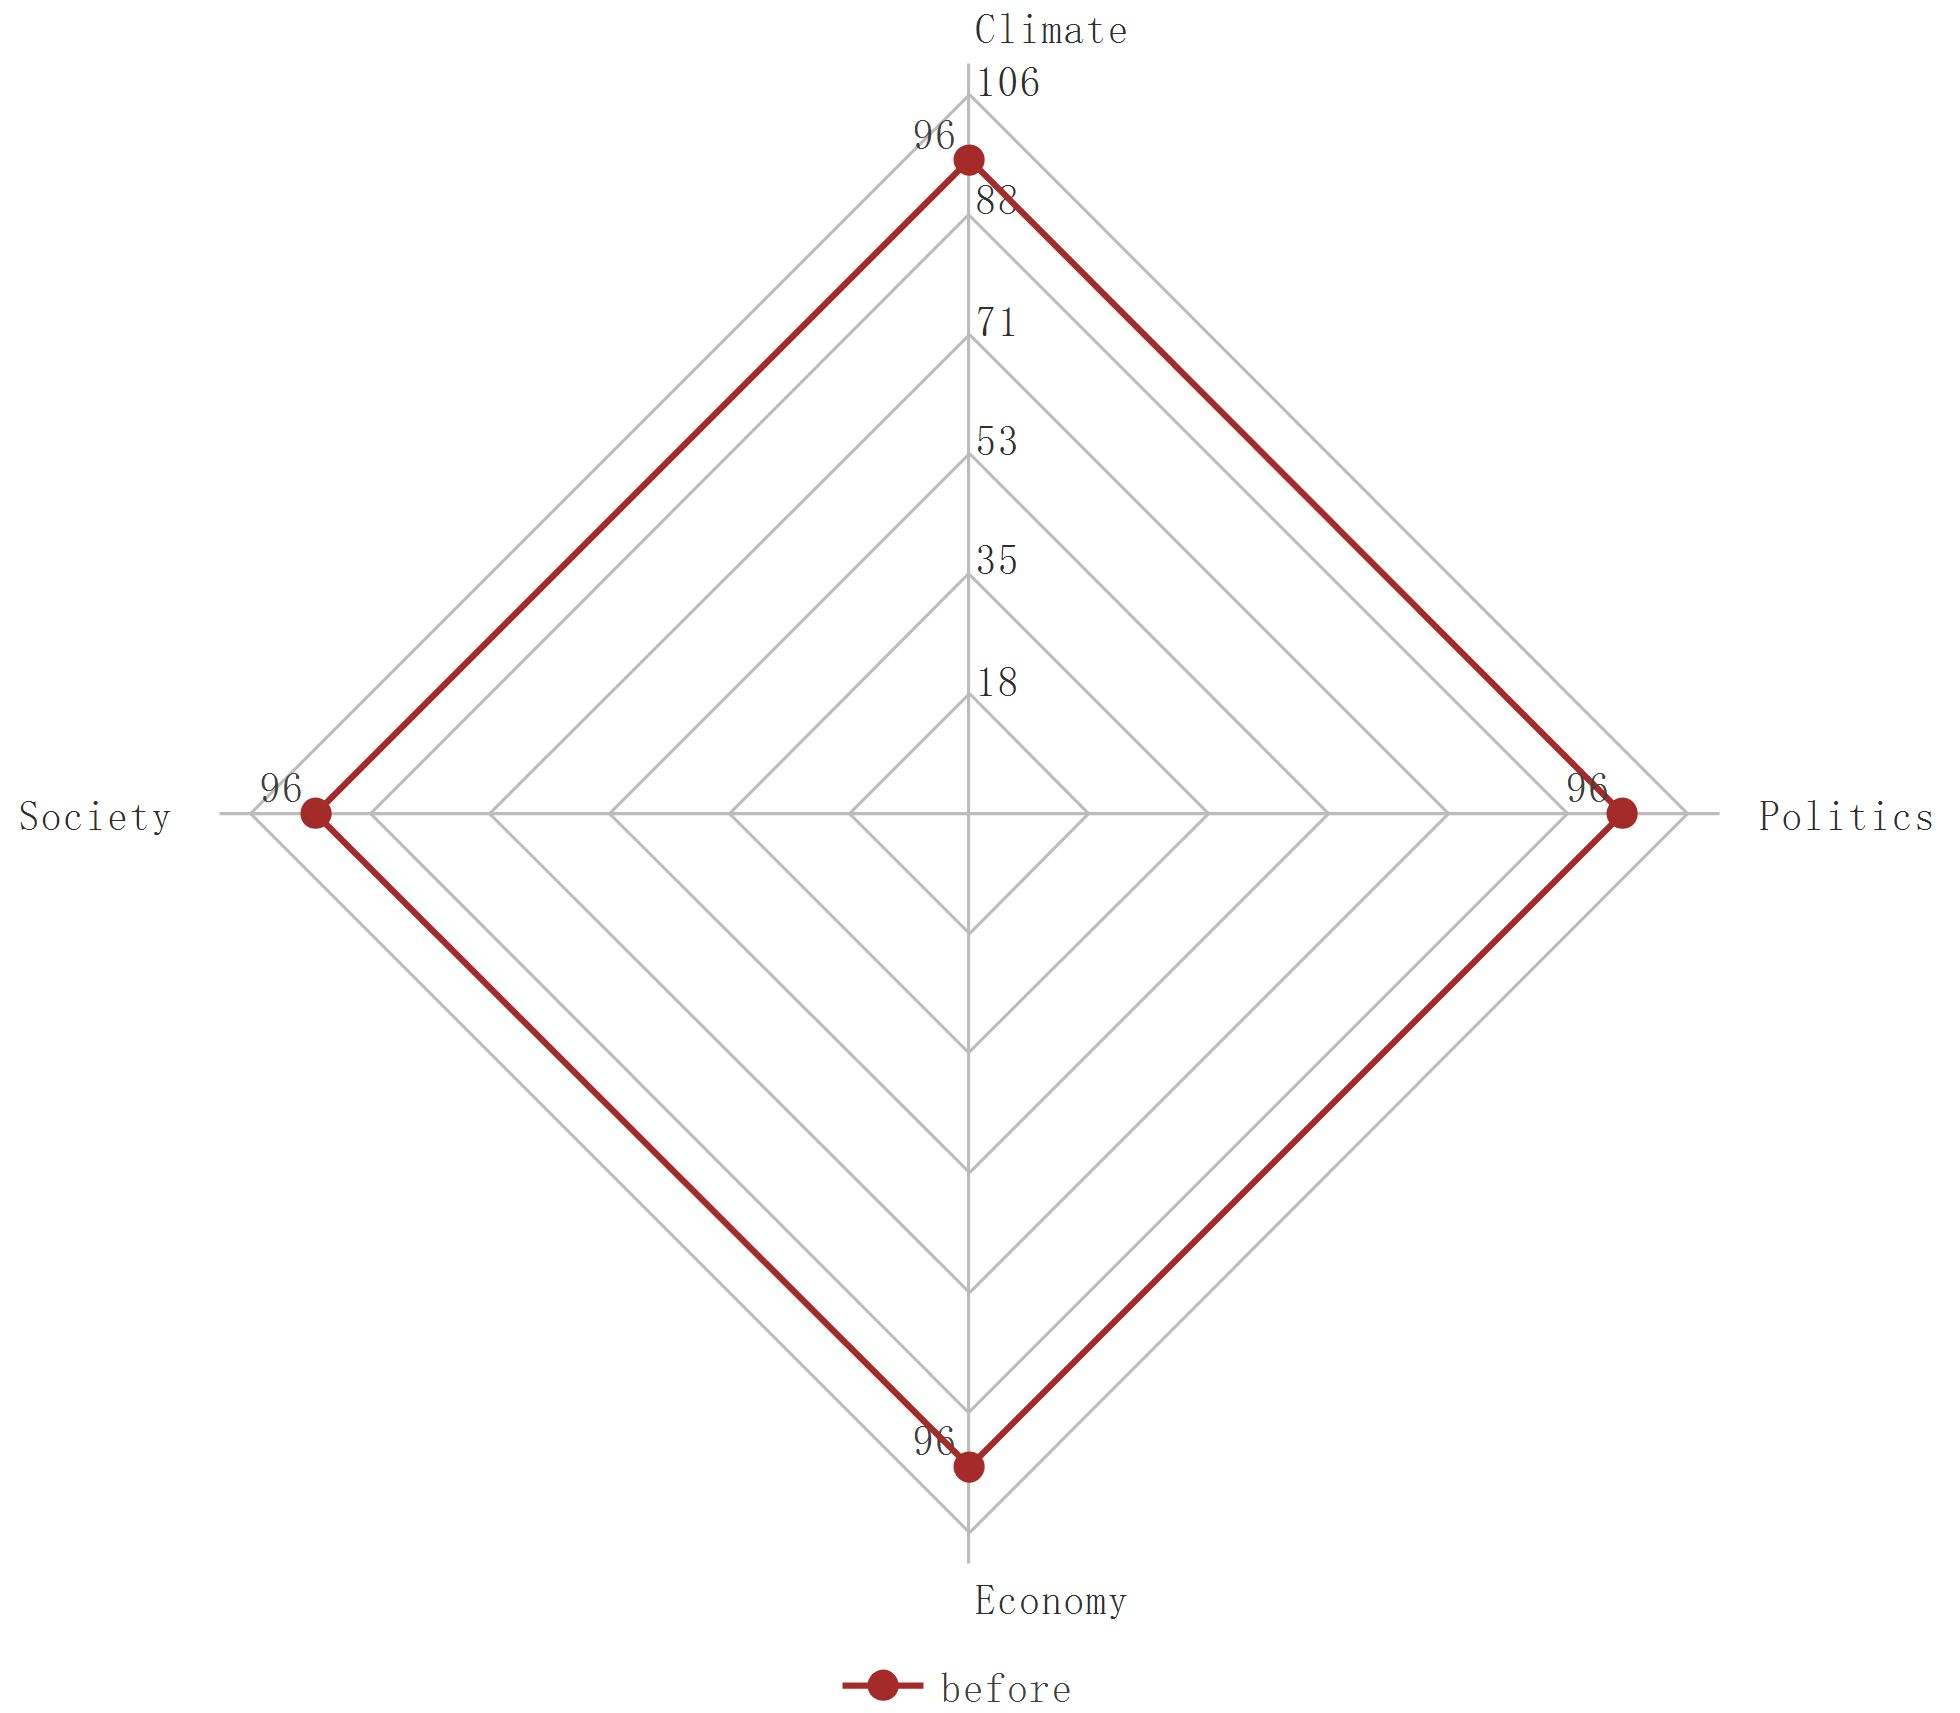
\includegraphics[width=2.5in]{yemen-1.jpg}
						%\caption{fig1}
					\end{minipage}%
				}%
				\subfigure[After]{
					\begin{minipage}[t]{0.5\linewidth}
						\centering
						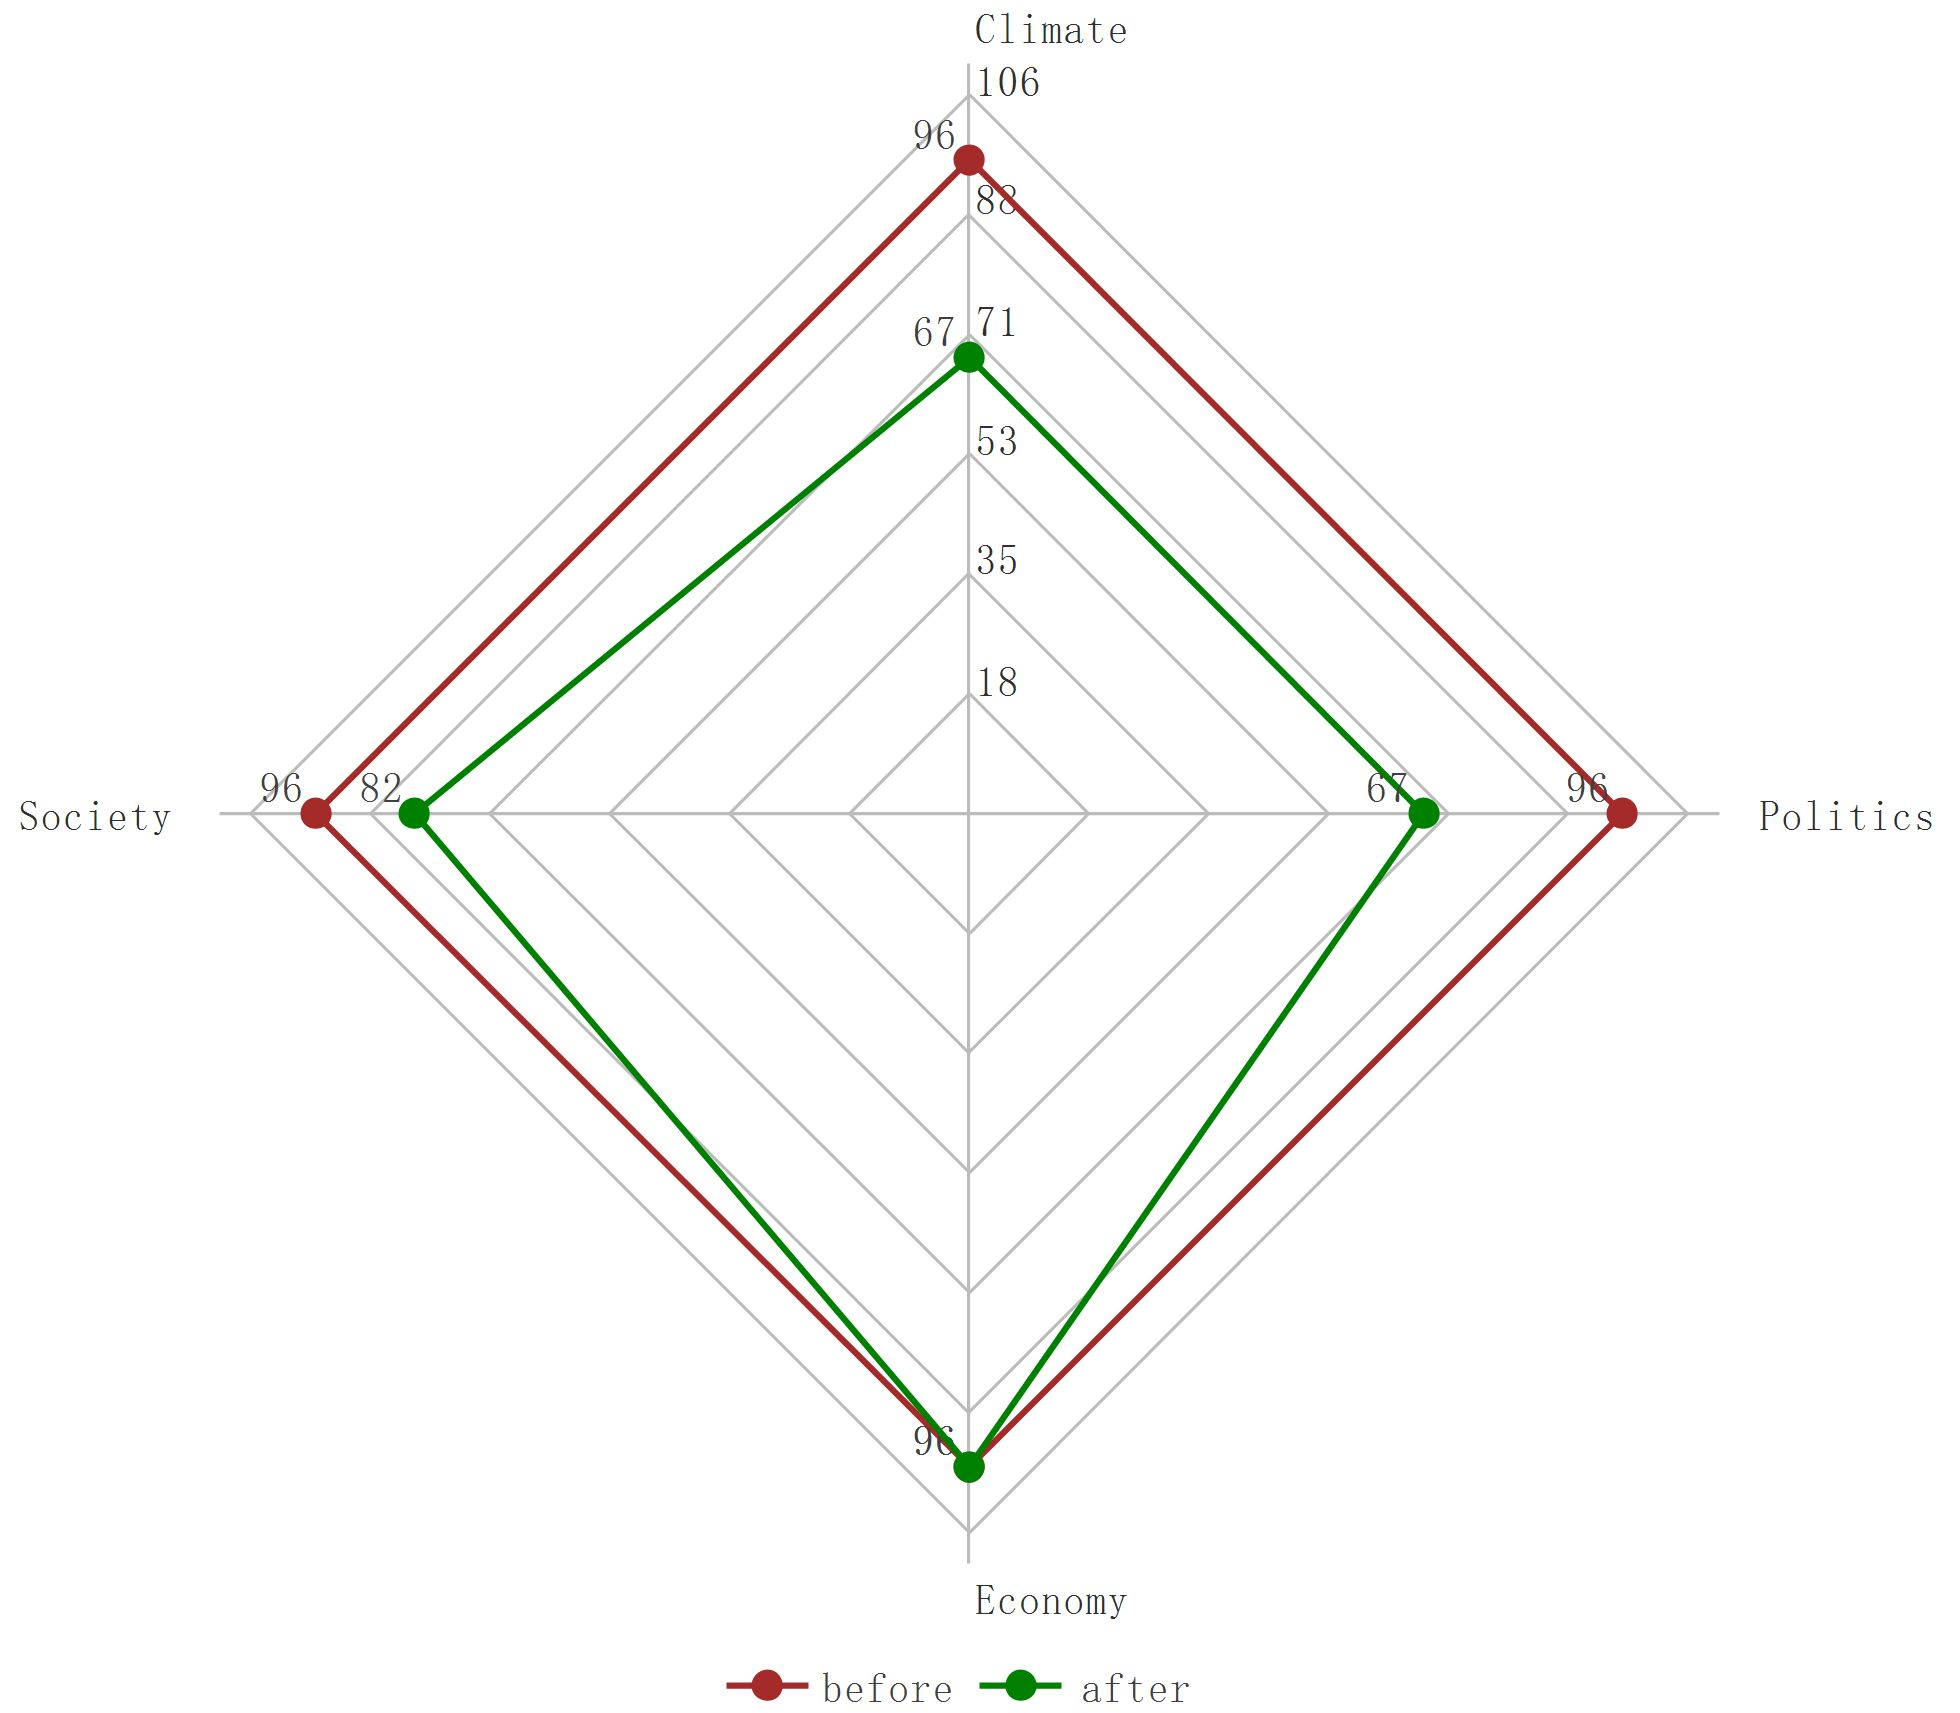
\includegraphics[width=2.5in]{yemen-2.jpg}
						%\caption{fig2}
					\end{minipage}%
				}%
				\centering
				\caption{Fragility Change without Climate Impact}
			\end{figure}
		
			The fragility before removing the climate impacts is 96,and it’s 80.1833 after removing the climate impacts. According to the categorization of our model, because Yemen's fragility was significantly reduced without the climate impacts , it has changed from fragile to vulnerable .
			
		\subsection{Anaylsis for Gabon}
		
			In this task, Gabon is selected as an object. In our model, the fragility index of Gabon is 88.945.  The reason why we choose Gabon is that it is in such a dangerous situation. With a slight impact of climate change, it can change from a vulnerable state to a fragile state.
			
			Through the data we collected from the internet as same as Yemen's data, we can see that Gabon has a very high forest cover rate. Its condition is much better than Yemen’s situation. 
			Based on our model, we sort the different climate change by impact, and the result is as follows:
			
			1. Forest area; 2. Arable land; 3. disaster; 4. Grain yield’s indirect influence through Intentional homicides; 5 Extreme climate’s indirect impact through political-competition; 6. Mean precipitation depth’s indirect impact through death caused by non-communicable diseases; 7. Extreme climate’s indirect impact through mean-years-of-schooling
			
			Through this rank, we can find that the indicator which has the most significant impact is Forest area. We define tipping points through our model. Tipping points are 77 and 89.5 which are the boundary of a different category. After it changed from 18.3484 to 18.9030, Gabon’s fragility changed from 88.945 to 89.5, which means it has evolved from vulnerable to fragile.
			
		
	\section{Human Intervention Model}
	
		Through the models we have established, we have found the impact of climate change on regional instability. Some of these effects are good, some are bad, some are direct, and some are implicit. Since the climate system is a complex system, it is unrealistic to control the climate to reduce national vulnerability directly. So we focus on those indicators that will be affected by climate change, in other words, we focus on the implicit impact of climate change. 
		
		So we will build a model to identify specific government interventions that can reduce the risk of climate change and measure the cost issues of government intervention.
		
		\begin{figure}[h]
			\small
			\centering
			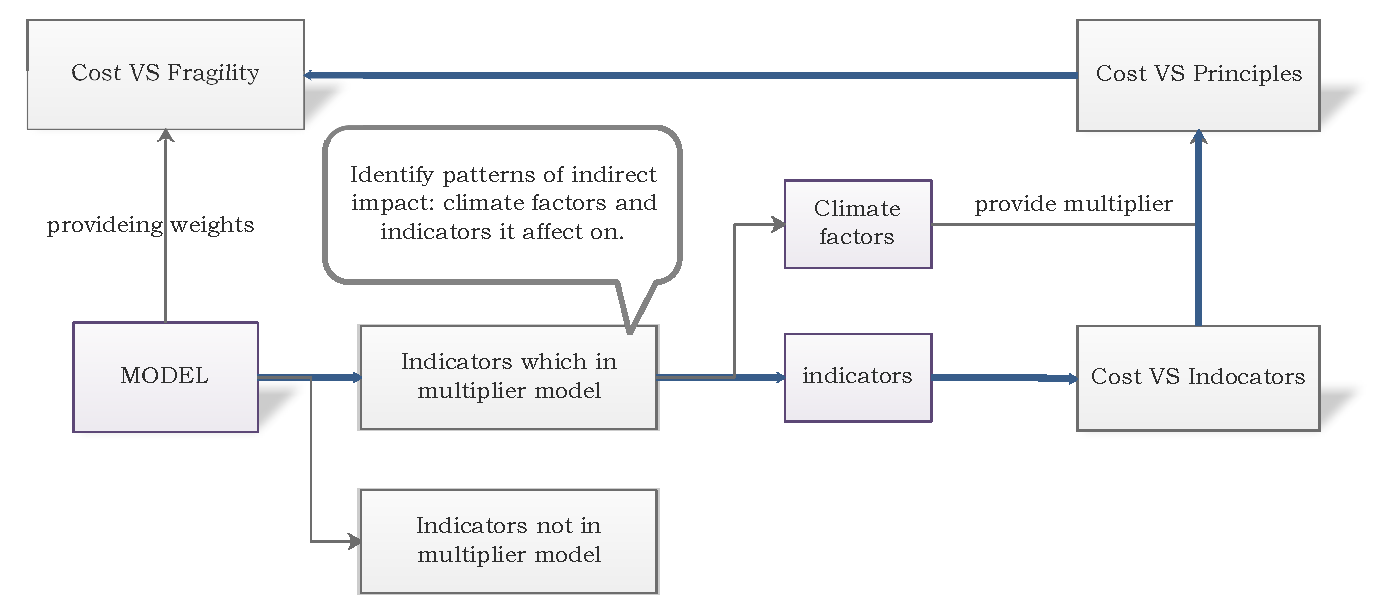
\includegraphics[width=14cm]{human-intervention.eps}
			\caption{Flow Chart of Human Intervention Model}
			\label{fig:human-intervention}
		\end{figure}
	
		\subsection{Cost Evaluation Model}
		
			\subsubsection{Assumptions}
	
				\begin{itemize}
					
					\item The Government considers the intervention method only according to the cost. When the government intervenes in a certain indicator, there are often many ways. We suppose that they will choose the most cost-effective solution.
					
					\item We use economic costs to calculate. The measures taken by the government to intervene in indicators will include multiple costs, such as human resource costs, but these can be measured in terms of money.
					
				\end{itemize}
			
			\subsubsection{Cost Evaluation Model}
			
			We use $X_i = \{ X_{1}, X_{2}, X_{3} \}$ to represent the three principals that are indirectly affected by the climate which are ECONOMICS, POLITICS and SOCIETY.
			
			It can be seen from our model that a total of six indicators will interact with climate change and further affect the fragility of the region. Let's use $a_{ij}$ to denote the j-th indicator which belong to principle $X_i$.

		
			\begin{equation}
				X _ { i } = \sum _ { j = 1 } ^{N} f _ { ij } ( a_{ij} , w_{ij} ) + C _ { i }
			\end{equation}
			
			$w_{ij}$ is a climatic implict indicators that can affect vulnerability through $a_{ij}$, and $ C _ { i }$ represent the contribution of other indicators on $X_i$.
			
			Through the data, we can find the relationship between the $c_{ij}$ and $\Delta a_{ij}$ where $c_{ij}$ denote the cost in $a_{ij}$ and $\Delta a_{ij}$ denote the change on $a_{ij}$:
			
			\begin{equation}
				\Delta a_{ij} = g _ { ij } \left( c _ { ij } \right)
			\end{equation}
			
			Based on this, we can measure the relationship between cost and principal changes.
			
			\begin{equation}
				\Delta X _ { i } = \sum_{j = 1}^{N} f _ { ij } \left( a_{ij} \left( c _ { ij } \right) , w \right)  - \sum_{j = 1}^{N} f _ { ij } \left( a_{ij} + g _ { ij } \left( c _ { ij } \right) , w \right)
			\end{equation}
			
			Based on the parameter settings determined by our previous model, we can calculate the change in the overall fragility of a region:
			
			\begin{equation}
				\Delta \text { Fragility } = \sum_{i=1}^3 \alpha_{i} \times \Delta X _ { i }
			\end{equation}
			
			So, we can calculate the total cost when the index of fragility needs to decrease $Q$ :
			
			\begin{equation}
			\begin{split}
			objective:& \quad \min S = \sum_{i} \sum_{ j } c _ { ij } \\
			s.t.:& \quad \Delta \text { Fragility } = Q \\
			& \quad c _ { ij } \geq 0
			\end{split}
			\end{equation}
		
		
		\subsection{Anaylsis for Gabon}
		
			We decide to keep on analyzing the task4 on the basis of Gabon. Because we cannot change the climate artificially, so we only consider interventions that would modify the index of indicators.
			
			
			Based on above analysation when its forest area index changed from 18.3484 to 18.9030, Gabon will be a fragile state. To mitigate the risk of climate change and prevent a country from becoming a fragile state, Gabon needs to take state driven interventions. After collecting cost data of interventions to different indicators, we found that only intentional homicides, mean-years-of-schooling and death caused by non-communicable diseases can be modified by interventions. 
			
			
			Based on Cost Evaluation Model we have made above, we take each interventions’ cost into consideration. Because no one wants to spend money in vain, so it’s not enough to only consider how much do these interventions cost, we also need to consider a best combination that would lead to a minimum cost. Which means that we need to solve an optimization problem.
			
			\begin{figure}[h]
				\small
				\centering
				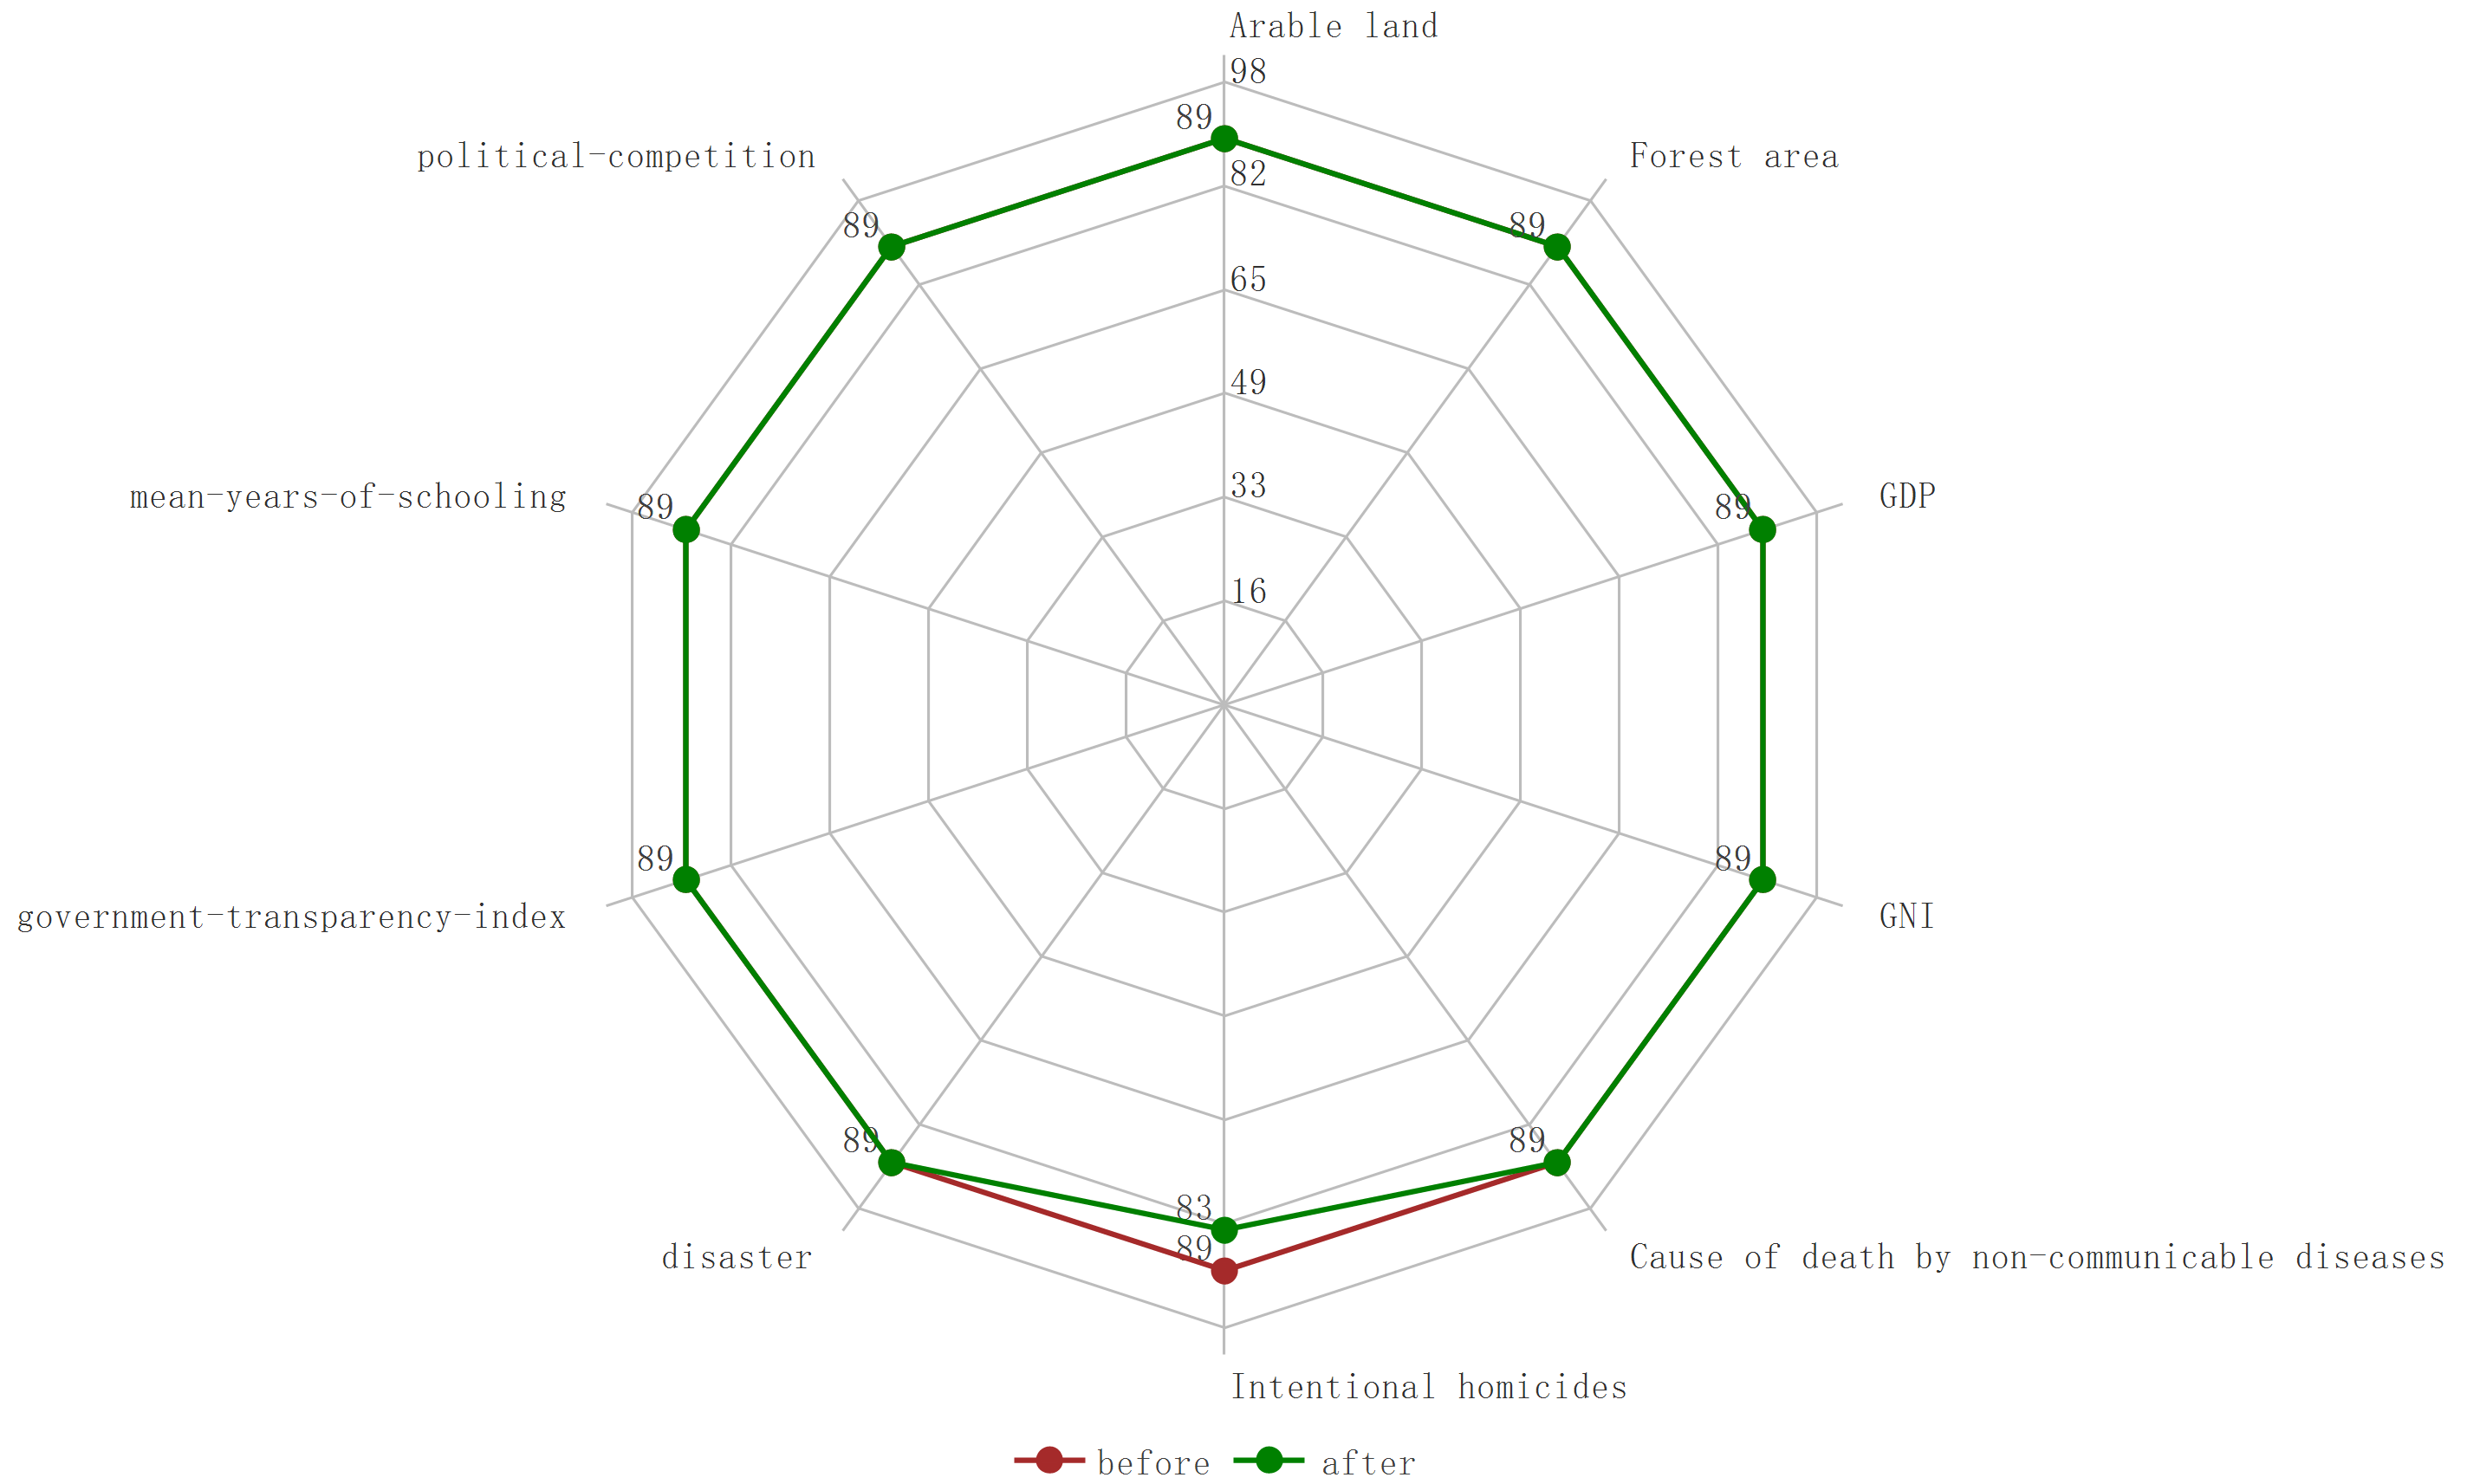
\includegraphics[width=14cm]{Gabon.png}
				\caption{Indicator change by Human Intervention}
				\label{fig:Gabon}
			\end{figure}
		
			\textbf{We use algorithm to solve the problem and find that only take state driven interventions to decrease intentional homicides is the best choice. This is the minimum cost solution. And it will cost about 3 billion which is the 20.9\% of the GDP.}
			
		
	
	\section{Sensitivity Analysis: Are models can fits different regional scale?}	
	
		Our model is essentially applicable to different regions' scale, such as cities or continents. To measure the fragility of a city or continent, the processes and ideas needed are the as same as the measurement of the country's instability. And part of the data can be modified to fit into the model with a simple operation. For example, national GDP data can be applied to the intercontinental through certain modifications. Political, economic, and social indicators for measuring countries can be applied to models that estimate cities.
		
		If we want to move the model successfully from a country-based to a city-based or continent-based, there are still some dilemmas and work that we need to consider. Below we consider the differences between country-based, continents-based and city-based models:
		
		\begin{itemize}
			
			\item From the perspective of model parameters, the parameters determined by country-based data cannot directly measure city or intercontinental instability.
			
			\item From the perspective of indicators, depending on the size of the region, the choice of the initial indicators will be different, some indicators should be revised, and some indicators should be deleted (some indicators that are meaningless at the city level, such as the number of national parties), some new indicators needed (indicators only meaningful at the continental scale).
			
			\item From the perspective of data, the data needs to be transformed to fit different level(Add or average), and some information needs to find an alternative.
			
		\end{itemize}
		
		
		The table \ref{fragility-indicators} given below is a comparison table of different regional scopes, and the national indicators are changed to obtain specific indicators suitable for different regions:
		
		
		\begin{table}[h]
			\caption{Indicators Suitable for Different Regions}
			\label{fragility-indicators}
			\centering
			\begin{tabular}{c | c | p{5cm}| p{5.8cm}}
					
				\specialrule{0.05em}{3pt}{3pt}
				 &country & city & continent\\
				\specialrule{0.05em}{3pt}{3pt}
				\multirow{10}{*}{Indicator}& AL & Get arable land (hectares per person) of each city	 & Per capita arable land data\\
				& FA	 & Get Forest of each city & 	Intercontinental total forest area divided by total continent area\\
				& DI & 	- & 	the number of disasters per continent\\
				& GTI	 & Municipal political transparency & 	-\\
				& PC & 	- & 	-\\
				& GDP & 	Urban production value & 	continent’s GDP\\
				& GNI & 	Total citizen income in the city & 	Total income of the continent\\
				& IH & 	City’s intentional homicide rate & 	Continent’s intentional homicide rate\\
				& DCBN & 	Non-communicable disease mortality in cities & Non-communicable disease mortality in continents\\
				& MYOS & 	Annual school enrollment rate in cities & 	Annual school enrollment rate in cities\\
				
				\specialrule{0.05em}{3pt}{3pt}
				\multirow{3}{*}{Added}&-&	Number of public facilities & -\\
				&-&	-&	Continental coastline length\\
				&-&	-&	Continental plate activity trend\\
				\specialrule{0.05em}{3pt}{3pt}

			\end{tabular}
		\end{table} 
		
		
		
	\clearpage
	
	
	\section{Strengths and Weaknesses}
	
		\subsection{Strengths}
		
			\begin{itemize}
				
				\item \textbf{Wide application}\\Our model is based on most countries’ data so that it can be applied to most countries.
				
				\item \textbf{Objective}\\Adopt a scientific weighting method (entropy weight method), so the weights we get are more credible.
				
				\item \textbf{Persuasive}\\We take a lot of factors into account, so our model is more plausible.
				
				\item \textbf{Vivid}\\We use different kinds of charts to explain our process and show our results.
		
			\end{itemize}
		
		\subsection{Weaknesses}
		
			\begin{itemize}
				
				\item \textbf{Lack of ability to deal with special problems}\\Lack of ability to deal with particular problems
				There might be some errors when our model is applied to some specific countries.
				
				\item \textbf{Loss of data source}\\We fill the missing data with the average magnitude of the continent which the state is located so there might be some experience errors.
				
				\item \textbf{Interpret Ability}\\The relation between indicators and second-class-indicators is based on common sense, so there might be some errors. 
				
			\end{itemize}
		
	\section{Future Work}
	
		Uncontrovertibly, there are many drawbacks in our model, such as the few data to analysis. We have to do a lot more to improve our work.
		
		\begin{itemize}
			
			\item \textbf{More data is needed}\\More statistical data will be needed in the future work, especially some extreme climate data and some long term climate change data. As a result, the prediction may not as precise as we anticipate
			
			\item \textbf{Analyze the fragility of country separately}\\We construct our model based on data from countries all around the world. But countries from continent to continent have much different conditions. So we need to analyze the data more separately, to measure the fragility more precisely. We should also analyze the data according to geographical distinction.
			
			\item \textbf{An interesting found}\\Our research has found that those fragile state’s condition tend to be worse, so those countries might be our priority to continue our work. Through the data we collected we found that the more fragile a state is, the less its statistical data could be collected. Unstable society, extreme poverty, low level of education makes it much more difficult to collect the data we need. So the absence of Statistical data itself reflects the fragility of a state to some extent. 
			
		\end{itemize}

	\nocite{*}
	\bibliography{reference}	
	\newpage


\end{document}
